\documentclass{amsart}
\usepackage{amsmath,amssymb,latexsym,color,ulem}
\usepackage[margin=1.5in]{geometry}
\usepackage{tikz}
\usepackage[bookmarks=true, bookmarksopen=true, bookmarksdepth=3,bookmarksopenlevel=2, colorlinks=true, linkcolor=blue, citecolor=blue, filecolor=blue, menucolor=blue, urlcolor=blue]{hyperref}

\usepackage[draft]{say}
\newcommand{\sayDR}[1]{\say[DR]{\color{red}{\bf DR:}\;#1}}
\newcommand{\saySS}[1]{\say[SS]{\color{blue}{\bf SS:}\;#1}}

\newtheorem{theorem}{Theorem}
\newtheorem{corollary}[theorem]{Corollary}
\newtheorem{definition}[theorem]{Definition}
\newtheorem{lemma}[theorem]{Lemma}
\newtheorem{proposition}[theorem]{Proposition}
\newtheorem{remark}[theorem]{Remark}
\newtheorem{question}{Question}

\numberwithin{theorem}{section}

\newcommand{\bfc}{\boldsymbol{c}}
\newcommand{\bfg}{\boldsymbol{g}}
\newcommand{\bfr}{\boldsymbol{r}}
\newcommand{\bfx}{\boldsymbol{x}}
\newcommand{\bfy}{\boldsymbol{y}}

\newcommand{\cC}{\mathcal{C}}
\newcommand{\cD}{\mathcal{D}}
\newcommand{\cI}{\mathcal{I}}
\newcommand{\cP}{\mathcal{P}}
\newcommand{\cQ}{\mathcal{Q}}

\newcommand{\fp}{\mathfrak{p}}

\newcommand{\CC}{\mathbb{C}}
\newcommand{\RR}{\mathbb{R}}
\newcommand{\TT}{\mathbb{T}}
\newcommand{\ZZ}{\mathbb{Z}}

\newcommand{\ol}[1]{{\overline{#1}}}
\newcommand{\vv}[1]{{{}^\vee \! #1}}

\newcommand{\Aut}{\operatorname{Aut}}
\newcommand{\Col}{\operatorname{Col}}
\newcommand{\diag}{\operatorname{diag}}
\newcommand{\dpt}{\operatorname{dp}}
\newcommand{\hgt}{\operatorname{ht}}
\newcommand{\Id}{\operatorname{Id}}
\newcommand{\into}{\hookrightarrow}
\newcommand{\obeta}{{\overline{\beta}}}
\newcommand{\oi}{{\overline{\imath}}}
\newcommand{\ot}{{\overline{t}}}
\newcommand{\rsh}{{\operatorname{rsh}}}
\newcommand{\sh}{{\operatorname{sh}}}
\newcommand{\WA}{{W\!\!A}}
\newcommand{\wt}{{\operatorname{wt}}}

\title{Dominance Regions for Imaginary $\bfg$-vectors}

\author{Dylan Rupel}
\author{Salvatore Stella}

\begin{document}
  \begin{abstract}
    We investigate the shapes of the polytopes defining the dominance order for $\bfg$-vectors in acyclic affine cluster algebras and acyclic cluster algebras of rank two.
    In both cases, we arrive at a complete description: 
    \begin{itemize}
      \item cluster monomials are never deformable;
      \item in affine types, the imaginary $\bfg$-vectors have dominance polytopes which are segments of imaginary $\bfg$-vectors except possibly for a single point on the boundary of an imaginary cone;
      \item a strange difference emerges in rank two wild types: the imaginary dominance polytopes are kites, triangles, or trapezoids which extend far outside the imaginary cone, the triangles appearing along rays corresponding to columns of the associated Cartan matrix.
    \end{itemize}
    We conjecture how our observations might generalize to higher dimensions.
  \end{abstract}
  \maketitle

  \section{Questions}
  \begin{enumerate}
    \item To what extent can we explicitly/combinatorially describe the eigenvalues/eigenvectors of the twist automorphism/Auslander-Reiten translation acting on imaginary $\bfg$-vectors given a maximal green sequence? 
    \item What role do coefficients play in the dominance order on pointed bases?
    \item Is any change required in the theory to handle quantum/generalized or both cases together?
    \item What do our results mean geometrically in terms of the cluster variety?
  \end{enumerate}

  \section{Introduction}
  The investigations of this paper are inspired by the dominance order on the tropical labelings for bases of cluster algebras.
  This dominance order is used by Qin to understand how these bases may be deformed in the case when there is a green-to-red sequence of mutations.
  In particular, these calculations can be carried out for any acyclic cluster algebra.

  Our calculations reveal the maximal support possible for a pointed basis which reproduces under mutations.
  In particular, any candidate basis can be ruled out using these results based upon their support alone.

  \section{Lattice Mutations and Linear Inequalities}
  Let $B=(b_{ij})$ be an $n\times n$ skew-symmetrizable integer matrix, i.e. there exists a diagonal integer matrix $D=\diag(d_1,\ldots,d_n)$ so that $DB$ is skew-symmetric, more precisely we have $d_i b_{ij}=-d_j b_{ji}$.
  Write $\Col(B)$ for the span of the columns of $B$ inside $\RR^n$ and $\Col^+(B)$ for their non-negative span.
  Define $\Col_\ZZ(B)$ and $\Col^+_\ZZ(B)$ analogously over the integers.

  The matrix $B$ is \emph{acyclic} if there is no sequence $i_1,\ldots,i_m,i_{m+1}=i_1$ so that $b_{i_\ell i_{\ell+1}}>0$ for $1\le\ell\le m$.
  This condition is naturally interpreted in terms of an associated quiver $Q_B$ with $n$ vertices and an arrow $i\to j$ whenever $b_{ji}>0$ (if we need to use representation theory at any point we'll have to change this to be $\gcd(b_{ij},b_{ji})$ arrows $i\to j$).
  Indeed, this is precisely the condition that $Q_B$ has no oriented cycles.
  In the case when $B$ is acyclic, there exists a labeling $\{k_1,\ldots,k_n\}=\{1,\ldots,n\}$ so that $\ell<\ell'$ implies $b_{k_{\ell'} k_\ell}\ge 0$.
  The sequence $(k_1,\ldots,k_n)$ (resp. $(k_n,\ldots,k_1)$) is then said to be \emph{source-adapted} (resp. \emph{sink-adapted}) since the condition implies $k_1$ is a source and $k_n$ is a sink in $Q_B$.
  %\sayDR{We need to pin down this convention.}

  For $b\in\ZZ$, write $[b]_+=max(b,0)$.
  Given a sign $\varepsilon\in\{\pm1\}$ and $k\in\{1,\ldots,n\}$, define a matrix $E_{k,\varepsilon}=(e_{ij})$ with
  \begin{equation}
    \label{eq:left mutation matrix}
    e_{ij}=\begin{cases} 1 & \text{if $i=j\ne k$;}\\ -1 & \text{if $i=j=k$;}\\ [\varepsilon b_{ik}]_+ & \text{if $i\ne j=k$;}\\ 0 & \text{otherwise;} \end{cases}
  \end{equation}
  and a matrix $F_{k,\varepsilon}=(f_{ij})$ with
  \begin{equation}
    \label{eq:right mutation matrix}
    f_{ij}=\begin{cases} 1 & \text{if $k\ne i=j$;}\\ -1 & \text{if $k=i=j$;}\\ [-\varepsilon b_{kj}]_+ & \text{if $k=i\ne j$;}\\ 0 & \text{otherwise.} \end{cases}
  \end{equation}
  Observe that $E^2_{k,\varepsilon}=\Id$ and $F^2_{k,\varepsilon}=\Id$ for any $k$ and any choice of $\varepsilon$.
  \begin{lemma}
    For $\varepsilon\in\{\pm1\}$ and $k\in\{1,\ldots,n\}$, we have $E_{k,-\varepsilon}E_{k,\varepsilon}=I_n+\varepsilon B^{\bullet k}$ and $E_{k,\varepsilon}-E_{k,-\varepsilon}=\varepsilon B^{\bullet k}$.
  \end{lemma}
  \begin{proof}
    This is immediate from the equality $\varepsilon b_{ij}=[\varepsilon b_{ij}]_+-[-\varepsilon b_{ij}]_+$.
  \end{proof}

  The index $k\in\{1,\ldots,n\}$ also determines a new skew-symmetrizable matrix $\mu_k B=(b'_{ij})$ given by
  \[ b'_{ij}=\begin{cases} -b_{ij} & \text{if $i=k$ or $j=k$;}\\ b_{ij}+[b_{ik}]_+b_{kj}+b_{ik}[-b_{kj}]_+ & \text{otherwise.} \end{cases} \]
  One easily observes that $\mu_k B$ is again skew-symmetrizable using the same matrix $D$.
  \begin{remark}
    Note that $\mu_k B=E_{k,\varepsilon} B F_{k,\varepsilon}$ for $\varepsilon=\pm 1$, the case $\varepsilon=1$ being obvious from the definitions and the case $\varepsilon=-1$ following from the identity $b_{ij}=[b_{ij}]_+-[-b_{ij}]_+$.
  \end{remark}

  To record sequences of these matrix mutations, we introduce the labeled $n$-regular rooted tree $\TT_n$ with root vertex $t_0$ and associate skew-symmetrizable matrices $B^t$ for $t\in\TT_n$ satisfying:
  \begin{itemize}
    \item $B^{t_0}=B$;
    \item if $t,t'\in\TT_n$ are joined by an edge labeled $k$, then $B^{t'}=\mu_k B^t$.
  \end{itemize}

  (DR: I changed to $\RR$ because it didn't seem like we really cared about integer points at the moment, when we try to link up with minors this will need to be added.)
  For $t\in\TT_n$, define $\phi^t_k:\RR^n\to\RR^n$ as the piecewise-linear map
  \[\phi^t_k(\lambda)=\begin{cases} E^t_{k,+}\lambda & \text{if $\lambda_k\ge0$;}\\ E^t_{k,-}\lambda & \text{if $\lambda_k<0$;} \end{cases}\]
  where the entries of $E^t_{k,\varepsilon}$ are given by \eqref{eq:left mutation matrix} with $b^t_{ij}$ in place of $b_{ij}$.
  We leave it as an exercise for the reader to check that $(\phi^t_k)^{-1}=\phi^{t'}_k$ whenever $t,t'\in\TT_n$ are joined by an edge labeled $k$.
  \begin{lemma}
    Suppose $t,t'\in\TT_n$ are joined by an edge labeled $k$.
    If $\mu\in\lambda+\Col(B^t)$, then $\phi^t_k(\mu)\in\phi^t_k(\lambda)+\Col(B^{t'})$.
  \end{lemma}
  \begin{proof}
    Suppose $\mu=\lambda+B^t\alpha$ for some $\alpha\in\RR^n$.
    Let $\varepsilon$ (resp. $\varepsilon'$) be such that $\phi^t_k(\mu)=E^t_{k,\varepsilon}\mu$ (resp. $\phi^t_k(\lambda)=E^t_{k,\varepsilon'}\lambda$).
    Then 
    \[\phi^t_k(\mu)=E^t_{k,\varepsilon}\mu=E^t_{k,\varepsilon}(\lambda+B^t\alpha)=E^t_{k,\varepsilon}\lambda + E^t_{k,\varepsilon} B^t F^t_{k,\varepsilon} F^t_{k,\varepsilon}\alpha=E^t_{k,\varepsilon}\lambda + B^{t'} F^t_{k,\varepsilon}\alpha.\]
    If $\varepsilon'=\varepsilon$, this is equal to $\phi^t_k(\lambda) + B^{t'} F^t_{k,\varepsilon}\alpha$ and so $\phi^t_k(\mu)\in\phi^t_k(\lambda)+\Col(B^{t'})$.
    Otherwise, 
    \[E^t_{k,\varepsilon}\lambda=E^t_{k,\varepsilon'}\lambda+\varepsilon(B^t)^{\bullet k}\lambda=\phi^t_k(\lambda)-\varepsilon(B^{t'})^{\bullet k}\lambda=\phi^t_k(\lambda)-\varepsilon B^{t'} \lambda_k \mathbf{e}_k\]
    and again we see that $\phi^t_k(\mu)\in\phi^t_k(\lambda)+\Col(B^{t'})$.
  \end{proof}

  For $t\in\TT_n$, define the piecewise-linear automorphisms $\phi_t:\RR^n\to\RR^n$ by
  \begin{itemize}
    \item $\phi_{t_0}=\Id$;
    \item if $t,t'\in\TT_n$ are joined by an edge labeled $k$, then $\phi_{t'}=\phi^t_k \phi_t$.
  \end{itemize}

  Suppose $B$ is acyclic.
  Given a sequence of signs $\varepsilon=(\varepsilon_1,\ldots,\varepsilon_n)$, define a quiver $Q_{B,\varepsilon}$ from $Q_B$ by removing all arrows starting at vertex $i$ whenever $\varepsilon_i=-1$.
  For $1\le j\le n$, define $\cP_j(Q_{B,\varepsilon})$ as the set of paths in $Q_{B,\varepsilon}$ starting at vertex $j$.
  Elements of $\cP_j(Q_{B,\varepsilon})$ are sequences of vertices $(p_1,\ldots,p_r)$ with $p_1=j$ and $b_{p_{t+1}p_t}>0$ for $1\le t\le r-1$.
  Given a path $p\in\cP_j(Q_{B,\varepsilon})$, a vertex $i\in Q_0$, and a sequence of signs $\varepsilon=(\varepsilon_1,\ldots,\varepsilon_n)$, set
  \[\wt_{i,\varepsilon}(p):=-b_{ip_r}^{(1-\delta_{ip_r})(1+\varepsilon_{p_r})/2}\prod_{t=1}^{r-1} b_{p_{t+1}p_t},\]
  where the prefactor $b_{ip_r}^{(1-\delta_{ip_r})(1+\varepsilon_{p_r})/2}$ is omitted if $i=p_r$ or $\varepsilon_{p_r}=-1$.
  \begin{lemma}
    Suppose $B$ is acyclic with source-adapted sequence $k_1,\ldots,k_n$.
    Consider $t_1,\ldots,t_n\in\TT_n$ so that $t_{\ell-1}$ is joined to $t_\ell$ by an edge in $\TT_n$ labeled by $k_\ell$ for $1\le\ell\le n$.
    For a sequence of signs $\varepsilon=(\varepsilon_1,\ldots,\varepsilon_n)$, the product $E^{t_{n-1}}_{k_n,\varepsilon_{k_n}}\cdots E^{t_0}_{k_1,\varepsilon_{k_1}}$ is given by $\tau=(\tau_{ij})$ with
    \begin{equation}
      \label{eq:tropical twist}
      \tau_{ij}=\sum_{p\in\cP_j(Q_{B,\varepsilon})}^* \wt_{i,\varepsilon}(p),
    \end{equation}
    where the $*$ indicates that the summation includes the trivial path at $j$ only if $i\le j$ when $\varepsilon_j=1$ and only if $i=j$ when $\varepsilon_j=-1$.

    Then $\phi_{t_n}$ is the following piecewise-linear automorphism:
    \begin{equation}
      \label{eq:tropical twist}
      \text{(This is going to require casework with the possible signs, we'll really only need it for imaginary $\bfg$-vectors though.)}
    \end{equation}
    The answer comes from selectively ``turning off'' arrows out of chosen vertices as indicated by choosing $\varepsilon_i=-1$.
  \end{lemma}
  \begin{proof}
    We prove the following modified formula for the product $E^{t_{n-1}}_{k_n,\varepsilon_{k_n}}\cdots E^{t_{m-1}}_{k_m,\varepsilon_{k_m}}$ for $1\le m\le n$ by reverse induction on $m$.
    Writing this matrix as $\tau^{(m)}=(\tau^{(m)}_{ij})$, we claim that
    \begin{equation}
      \label{eq:tropical twist}
      \tau^{(m)}_{ij}=\begin{cases} \sum\limits_{p\in\cP_j(Q_{B,\varepsilon}^{(m)})}^* \wt_{i,\varepsilon}(p) & \text{if $j=k_\ell$ with $m\le\ell$;}\\ \delta_{ij} & \text{otherwise;} \end{cases}
    \end{equation}
    where $Q_{B,\varepsilon}^{(m)}$ is the full subquiver of $Q_{B,\varepsilon}$ on vertices $k_m,\ldots,k_n$.
    Note that the weight function follows the same definition as above.

    Since the sequence $k_1,\ldots,k_n$ is source-adapted, the matrix $E^{t_{m-1}}_{k_m,\varepsilon_m}$, for $1\le m\le n$, has entries $e^{(m)}_{ij}$ given by
    \begin{equation}
      \label{eq:source mutation matrix}
      e^{(m)}_{ij}=\begin{cases} 1 & \text{if $i=j\ne k_m$;}\\ -1 & \text{if $i=j=k_m$;}\\ [-\varepsilon_{k_m} b_{ik_m}]_+ & \text{if $i=k_\ell$, $j=k_m$, $\ell<m$;}\\ [\varepsilon_{k_m} b_{ik_m}]_+ & \text{if $i=k_\ell$, $j=k_m$, $m<\ell$;}\\ 0 & \text{otherwise;} \end{cases}
    \end{equation}
    the entries for $\ell<m$ picking up the sign from the prior matrix mutations.

    For $m=n$, it is clear that $\tau^{(n)}_{ij}=e^{(n)}_{ij}$ for $j\ne k_n$.
    If $\varepsilon_{k_n}=1$, there is only the trivial path $(k_n)$ in $Q_{B,\varepsilon}^{(n)}$ and we have $\tau^{(n)}_{ik_n}=-b_{ik_n}$, which agrees with $e^{(n)}_{ik_n}$ in this case.
    Otherwise, $\varepsilon_{k_n}=-1$ and the sum is empty for $i\ne k_n$ giving $\tau^{(n)}_{ik_n}=0=e^{(n)}_{ik_n}$ or only takes the trivial path for $i=k_n$ giving $\tau^{(n)}_{k_nk_n}=-1=e^{(n)}_{k_nk_n}$.
    This gives the base of the induction.

    Now suppose the matrix $\tau^{(m)}$ is given as above.
    Using equation \eqref{eq:source mutation matrix}, we need to check that 
    \begin{equation}
      \label{eq:twist matrix recursion}
      \tau^{(m-1)}_{ij}=\sum\limits_{p=1}^n \tau^{(m)}_{ip} e^{(m-1)}_{pj}=\begin{cases} \tau^{(m)}_{ij} & \text{if $j\ne k_{m-1}$;}\\ -\tau^{(m)}_{ik_{m-1}} + \sum\limits_{\ell=1}^{m-2} \tau^{(m)}_{i k_\ell} [-\varepsilon_{k_{m-1}} b_{k_\ell k_{m-1}}]_+ + \sum\limits_{\ell=m}^n \tau^{(m)}_{i k_\ell} [\varepsilon_{k_{m-1}} b_{k_\ell k_{m-1}}]_+ & \text{if $j=k_{m-1}$;}\end{cases}
    \end{equation}
    is computed by the formula above.
    First observe that $\tau^{(m-1)}_{ij}=\tau^{(m)}_{ij}=\delta_{ij}$ if $j=k_\ell$ with $\ell<m-1$.  
    Second observe that $\cP_j(Q_{B,\varepsilon}^{(m-1)})=\cP_j(Q_{B,\varepsilon}^{(m)})$ whenever $j=k_\ell$ with $m\le\ell$, i.e. the purported formulas for $\tau^{(m-1)}_{ij}$ and $\tau^{(m)}_{ij}$ agree in this case.
    Therefore it remains to show that
    \[
      \tau^{(m-1)}_{i k_{m-1}}=-\delta_{ik_{m-1}} + \sum\limits_{\ell=1}^{m-2} \delta_{i k_\ell} [-\varepsilon_{k_{m-1}} b_{k_\ell k_{m-1}}]_+ + \sum\limits_{\ell=m}^n \sum\limits_{p\in\cP_{k_\ell}(Q_{B,\varepsilon}^{(m)})}^* \wt_{i,\varepsilon}(p) [\varepsilon_{k_{m-1}} b_{k_\ell k_{m-1}}]_+
    \]
    agrees with the desired expression.
    Indeed, for $\varepsilon_{k_{m-1}}=-1$ this reduces to $\tau^{(m-1)}_{i k_{m-1}}=-\delta_{i k_{m-1}}$ which matches with the desired expression in this case.
    Then assuming $\varepsilon_{k_{m-1}}=1$, we are comparing with
    \[
      \tau^{(m-1)}_{i k_{m-1}}=-\delta_{ik_{m-1}} - \sum\limits_{\ell=1}^{m-2} \delta_{i k_\ell} b_{k_\ell k_{m-1}} + \sum\limits_{\ell=m}^n \sum\limits_{p\in\cP_{k_\ell}(Q_{B,\varepsilon}^{(m)})}^* \wt_{i,\varepsilon}(p) b_{k_\ell k_{m-1}}.
    \]
    But observe that the final summation above contributes the nontrivial paths to the summation $\sum\limits_{p\in\cP_{k_{m-1}}(Q_{B,\varepsilon}^{(m-1)})}^* \wt_{i,\varepsilon}(p)$ while the first two terms above give the contribution, depending on $i$, corresponding to the trivial path $(k_{m-1})$.
  \end{proof}
  \begin{question}
    Is the trace of $\tau$ an invariant of matrix mutations?  P.A.: It is invariant under sink and source mutations since the trace is a class function and these mutations simply enact a cyclic shift in the factors of $\tau$.
  \end{question}

  For $\lambda\in\RR^n$, define the \emph{$B_t$-cone} $\cC_t(\lambda):=\lambda+B_t\cdot\RR_{\ge0}^n$ pointed at $\lambda$.
  \begin{definition}
    For $\lambda\in\RR^n$, define the \emph{dominance region} 
    \[ \cP(\lambda) = \bigcap_{t\in\TT_n} \phi_t^{-1} \cC_t(\phi_t \lambda). \]
    When $\mu\in\cP(\lambda)$, we say \emph{$\lambda$ dominates $\mu$}.
  \end{definition}
  Our goal is to understand the dominance polytopes $\cP(\lambda)$ for all $\lambda$.
  \begin{lemma}
    The sets $\cP(\lambda)$ are polytopes.
  \end{lemma}


  \begin{lemma}
    \label{le:transformed inequalities}
    Let $A$ be an invertible $n\times n$ matrix.
    Under the left action of $A$, say $A\bfx=\bfy$ for $\bfx,\bfy\in\RR^n$, the region inside $\RR^n$ defined by the inequality $\bfr\bullet(\bfx-\lambda)\le t$ with $\lambda,\bfr\in\RR^n$ and $t\in\RR$ is transformed into the region defined by the inequality \[(A^{-T}\bfr)\bullet(\bfy-A\lambda)\le t.\]
  \end{lemma}
  \begin{proof}
    This is immediate from the equalities
    \[\bfr\bullet(\bfx-\lambda)=\bfr^T(\bfx-\lambda)=\bfr^TA^{-1}A(\bfx-\lambda)=(A^{-T}\bfr)^T(A\bfx-A\lambda)=(A^{-T}\bfr)\bullet(\bfy-A\lambda).\]
  \end{proof}


  \section{Affine Types}
  Associated to an acyclic skew-symmetrizable matrix $B=(b_{ij})$ there is a Cartan matrix $A=(a_{ij})$ with $a_{ii}=2$ and $a_{ij}=-|b_{ij}|$.
  We say that $B$ is of affine type if its associated Cartan matrix gives rise to an affine Dynkin diagram.
  In this section, we focus on understanding the dominance polytopes for affine matrices $B$.

  Let $B=(b_{ij})$ be an $n\times n$ skew-symmetrizable matrix of affine type with associated Cartan matrix $A=(a_{ij})$.
  
  \begin{lemma}
    One column is always in the positive span of the other columns.
  \end{lemma}

  \begin{definition}
    Describe imaginary $\bfg$-vectors and those corresponding to cluster monomials.
  \end{definition}

  \begin{lemma}
    Let $\lambda\in\ZZ^n$ correspond to a cluster monomial.
    Then $\cP(\lambda)=\{\lambda\}$.
  \end{lemma}
  \begin{proof}
    An explicit sequence of sink/source mutations should suffice.
  \end{proof}

  

  \section{Rank Two}
  Fix integers $b,c>0$ and assume $bc\ge 4$.
  Let $B=\left[ \begin{array}{cc} 0 & -b \\ c & 0 \end{array} \right]$.
  Here we may take the 2-regular tree $\TT_2$ to have vertices labeled $t_i$ for $i\in\ZZ$, with $t_{2j}$ joined to $t_{2j+1}$ by an edge labeled $1$ and $t_{2j-1}$ joined to $t_{2j}$ by an edge labeled $2$.
  We aim to understand the dominance regions $\cP(\lambda) = \bigcap_{i\in\ZZ} \phi_{t_i}^{-1} \cC_{t_i}(\phi_{t_i} \lambda)$ for $\lambda\in\ZZ^2$.

  Observe that $\phi_{t_1}:=\phi_1^{t_0}$ is the piecewise-linear map given by
  \begin{equation}
    \label{eq:forward mutation 1}
    \phi_{t_1}(\lambda)=\begin{cases} (-\lambda_1,c\lambda_1+\lambda_2) & \text{if $\lambda_1\ge0$;}\\ (-\lambda_1,\lambda_2) & \text{if $\lambda_1<0$;} \end{cases}
  \end{equation}
  and $\phi_{t_2}:=\phi_2^{t_1}\phi_1^{t_0}$ is the piecewise-linear map given by
  \begin{equation}
    \label{eq:forward two step mutation}
    \phi_{t_2}(\lambda)=\begin{cases} \big((bc-1)\lambda_1+b\lambda_2, -c\lambda_1-\lambda_2\big) & \text{if $\lambda_1\ge 0$ and $c\lambda_1+\lambda_2\ge 0$;}\\ (-\lambda_1, -c\lambda_1-\lambda_2) & \text{if $\lambda_1\ge 0$ and $c\lambda_1+\lambda_2<0$;}\\ (-\lambda_1+b\lambda_2, -\lambda_2) & \text{if $\lambda_1<0$ and $\lambda_2\ge 0$;}\\ (-\lambda_1,-\lambda_2) & \text{if $\lambda_1<0$ and $\lambda_2<0$;}\end{cases}
  \end{equation}
  while $\phi_{t_2}^{-1}=\phi_{t_{-2}}$ is the piecewise-linear map given by
  \begin{equation}
    \label{eq:backward two step mutation}
    \phi_{t_2}^{-1}(\lambda)=\begin{cases} \big(-\lambda_1-b\lambda_2, c\lambda_1+(bc-1)\lambda_2\big) & \text{if $\lambda_2\le 0$ and $\lambda_1+b\lambda_2\le 0$;}\\ (-\lambda_1-b\lambda_2, -\lambda_2) & \text{if $\lambda_2\le 0$ and $\lambda_1+b\lambda_2>0$;}\\ (-\lambda_1, c\lambda_1-\lambda_2) & \text{if $\lambda_2>0$ and $\lambda_1\le 0$;}\\ (-\lambda_1,-\lambda_2) & \text{if $\lambda_2>0$ and $\lambda_1>0$;}\end{cases}
  \end{equation}

  By an eigenvector of a piecewise-linear map $\phi$, we will mean a vector $\lambda$ such that for each $k\ge0$, there exists a scalar $\nu_k$ so that $\phi^k(\lambda)=\nu_k\lambda$.
  \begin{lemma}
    Any nonzero eigenvector of $\phi_{t_2}$ is a positive multiple of one of the vectors $\big(2b,-bc\pm\sqrt{bc(bc-4)}\big)$.
  \end{lemma}
  \begin{proof}
    First observe that the equation $\phi_{t_2}^k(\lambda)=\nu_k\lambda$ cannot be satisfied for all $k\ge0$ unless $\lambda_1\ge 0$ and $c\lambda_1+\lambda_2\ge 0$.
    In this region, $\phi_{t_2}$ is linear with eigenvalue $\nu$ satisfying $\nu^2-(bc-2)\nu+1=0$, i.e. $\nu=\frac{bc-2\pm\sqrt{bc(bc-4)}}{2}$.
    We thus require that 
    \[\frac{bc-2\pm\sqrt{bc(bc-4)}}{2}\lambda_1=(bc-1)\lambda_1+b\lambda_2 \qquad\text{and}\qquad \frac{bc-2\pm\sqrt{bc(bc-4)}}{2}\lambda_2= -c\lambda_1-\lambda_2,\]
    or, equivalently, that
    \[\frac{-bc\pm\sqrt{bc(bc-4)}}{2b}\lambda_1=\lambda_2 \qquad\text{and}\qquad \frac{-bc\mp\sqrt{bc(bc-4)}}{2c}\lambda_2=\lambda_1.\]
    As these represent the same relation, the result immediately follows by inspection.
  \end{proof}

  Write $\cI \subset \RR^2$ for the \emph{imaginary cone} (positively) spanned by the vectors $\big(2b,-bc\pm\sqrt{bc(bc-4)}\big)$.
  Also, write $\cI' \subset \RR^2$ for the \emph{dual imaginary cone} (positively) spanned by the vectors $\big(-bc\pm\sqrt{bc(bc-4)},2c\big)$.
  \begin{lemma}
    The vectors $\big(2b, -bc+\sqrt{bc(bc-4)}\big)$ (resp. $\big(2b, -bc-\sqrt{bc(bc-4)}\big)$) and $\big(2c, bc+\sqrt{bc(bc-4)}\big)$ (resp. $\big(2c, bc-\sqrt{bc(bc-4)}\big)$) are perpendicular.
  \end{lemma}
  \begin{proof}
    This is immediate from the equality $\big(-bc+\sqrt{bc(bc-4)}\big)\big(bc+\sqrt{bc(bc-4)}\big)=-4bc$.
  \end{proof}
  \begin{lemma}
    \label{le:imaginary stability}
    For $j\in\ZZ$ and $\lambda\in\cI$, we have $\phi_{t_{2j}}(\lambda)\in\cI$ and $\phi_{t_{2j+1}}(\lambda)\in\cI'$.
  \end{lemma}
  \begin{proof}
    Note that $\phi_{t_{2j}}=\phi_{t_2}^j$ and $\phi_{2j+1}=\phi_{t_1}\phi_{t_2}^j$ so the result follows from the cases $j=1$ and $j=0$, respectively.
    The claim is immediate for $\phi_{t_2}$ since the vectors $\big(2b,-bc\pm\sqrt{bc(bc-4)}\big)$ are eigenvectors and $\phi_{t_2}$ is linear in $\cI$.
    Now, since $b>0$, we have $\phi_{t_1}(\lambda)=(-\lambda_1,c\lambda_1+\lambda_2)$ and so $\phi_{t_1}\Big( \big(2b,-bc\pm\sqrt{bc(bc-4)}\big) \Big)=\big(-2b,bc\pm\sqrt{bc(bc-4)}\big)$, which is the $\frac{bc\pm\sqrt{bc(bc-4)}}{2c}$-multiple of the boundary vector for $\cI'$ and the result follows for arbitrary $\lambda\in\cI$ by linearity of $\phi_{t_1}$ in this region.
  \end{proof}

  It will be useful to have explicit expressions for $\phi_{t_i}(\lambda)$ for $\lambda\in\cI$.
  For this, we define \emph{two-parameter Chebyshev polynomials} $u_{i,\varepsilon}$ for $i\in\ZZ$ and $\varepsilon\in\{\pm\}$ recursively by
  \[u_{0,\varepsilon}=0,\quad u_{1,\varepsilon}=1,\quad u_{i+1,\varepsilon}=\begin{cases} bu_{i,-\varepsilon}-u_{i-1,\varepsilon} & \text{if $\varepsilon=+$;}\\ cu_{i,-\varepsilon}-u_{i-1,\varepsilon} & \text{if $\varepsilon=-$.} \end{cases}\]
  Observe that, by an easy induction, $u_{-i,\varepsilon}=-u_{i,\varepsilon}$.

  The recursion can be written more succinctly as $u_{i+1,\varepsilon}=u_{2,\varepsilon}u_{i,-\varepsilon}-u_{i-1,\varepsilon}$ with the additional initial condition $u_{2,\varepsilon}=\begin{cases} b & \text{if $\varepsilon=+$;}\\ c & \text{if $\varepsilon=-$.} \end{cases}$
  This leads to the following more general recursive structure.
  \begin{lemma}
    For $i,\ell\in\ZZ$ and $\varepsilon\in\{\pm\}$, we have
    \begin{equation}
      \label{eq:long Chebyshev recursion}
      u_{i+\ell,\varepsilon}=\begin{cases} u_{\ell+1,\varepsilon}u_{i,-\varepsilon}-u_{\ell,-\varepsilon}u_{i-1,\varepsilon} & \text{\upshape if $\ell$ is odd;}\\ u_{\ell+1,-\varepsilon}u_{i,\varepsilon}-u_{\ell,\varepsilon}u_{i-1,-\varepsilon} & \text{\upshape if $\ell$ is even.} \end{cases}
    \end{equation}
  \end{lemma}
  \begin{proof}
    We work by induction on $\ell$, the cases $\ell=0,1$ being tautological and reproducing the defining recursion, respectively.
    Using the claim for $j>0$ and then the defining recursion twice, we get
    \begin{align*}
      u_{i+\ell+1,\varepsilon}&=\begin{cases} u_{\ell+1,\varepsilon}u_{i+1,-\varepsilon}-u_{\ell,-\varepsilon}u_{i,\varepsilon} & \text{if $\ell$ is odd;}\\ u_{\ell+1,-\varepsilon}u_{i+1,\varepsilon}-u_{\ell,\varepsilon}u_{i,-\varepsilon} & \text{if $\ell$ is even;} \end{cases}\\
      &=\begin{cases} (u_{2,-\varepsilon}u_{\ell+1,\varepsilon}-u_{\ell,-\varepsilon})u_{i,\varepsilon}-u_{\ell+1,\varepsilon}u_{i-1,-\varepsilon} & \text{if $\ell$ is odd;}\\ (u_{2,\varepsilon}u_{\ell+1,-\varepsilon}-u_{\ell,\varepsilon})u_{i,-\varepsilon}-u_{\ell+1,-\varepsilon}u_{i-1,\varepsilon} & \text{if $\ell$ is even;} \end{cases}\\
      &=\begin{cases} u_{\ell+2,-\varepsilon}u_{i,\varepsilon}-u_{\ell+1,\varepsilon}u_{i-1,-\varepsilon} & \text{if $\ell+1$ is even;}\\ u_{\ell+2,\varepsilon}u_{i,-\varepsilon}-u_{\ell+1,-\varepsilon}u_{i-1,\varepsilon} & \text{if $\ell+1$ is odd;} \end{cases}
    \end{align*}
    which is the claimed recursion for $\ell+1$.
    These calculations can be reversed to show the result for $\ell<0$.
  \end{proof}

  The following gives the desired expressions for $\phi_{t_i}(\lambda)$ when $\lambda\in\cI$.
  \begin{lemma}
    \label{le:imaginary transformations}
    For $j\in\ZZ$ and $\lambda\in\cI$, we have
    \begin{align*}
      \phi_{t_{2j}}(\lambda)&=(u_{2j+1,+}\lambda_1+u_{2j,+}\lambda_2,-u_{2j,-}\lambda_1-u_{2j-1,-}\lambda_2);\\
      \phi_{t_{2j+1}}(\lambda)&=(-u_{2j+1,+}\lambda_1-u_{2j,+}\lambda_2,u_{2j+2,-}\lambda_1+u_{2j+1,-}\lambda_2).
    \end{align*}
  \end{lemma}
  \begin{proof}
    We work by induction on $j$, the case $j=0$ being clear from the definitions.
    As observed above, we have $\phi_{t_{2j}}=\phi_{t_2}^j$.
    For $\lambda\in\cI$, the action of $\phi_{t_2}$ from \eqref{eq:forward two step mutation} can be rewritten as
    \[\phi_{t_2}(\lambda)=(u_{3,-}\lambda_1+u_{2,+}\lambda_2,-u_{2,-}\lambda_1-u_{1,+}\lambda_2),\]
    and so
    \begin{align*}
      \phi_{t_{2j+2}(\lambda)}&=\phi_{t_2}\phi_{t_{2j}}(\lambda)\\
      &=\big( (u_{3,-}u_{2j+1,+}-u_{2,+}u_{2j,-})\lambda_1+(u_{3,-}u_{2j,+}-u_{2,+}u_{2j-1,-})\lambda_2,\\
      &\qquad -(u_{2,-}u_{2j+1,+}-u_{1,+}u_{2j,-})\lambda_1-(u_{2,-}u_{2j,+}-u_{1,+}u_{2j-1,-})\lambda_2 \big)\\
      &=(u_{2j+3,+}\lambda_1+u_{2j+2,+}\lambda_2, -u_{2j+2,-}\lambda_1-u_{2j+1,-}\lambda_2),
    \end{align*}
    as desired, where the last equality uses \eqref{eq:long Chebyshev recursion} with $i=2j+1$ and $\ell=2$.

    Similarly, using $\phi_{t_1}(\lambda)=(-\lambda_1,u_{2,-}\lambda_1+u_{1,+}\lambda_2)$ for $\lambda\in\cI$, together with the basic Chebyshev recursion and the equality $\phi_{2j+1}=\phi_{t_1}\phi_{t_2}^j$ gives the claimed formula for $\phi_{t_{2j+1}}$ from that of $\phi_{t_{2j}}$.
  \end{proof}

  Next we aim to understand how inequalities transform under the action of a linear map, this will be the key tool for describing the dominance regions $\cP(\lambda)$ for $\lambda\in\cI$.
  \begin{lemma}
    \label{le:transformed inequalities}
    Let $A=(a_{ij})$ be an invertible $2\times 2$ matrix.
    Under the action of $A$, the region inside $\RR^2$ defined by the inequality $rx+sy\le t$ is transformed to the region defined by the inequality \[\frac{ra_{22}-sa_{21}}{a_{11}a_{22}-a_{12}a_{21}}x + \frac{-ra_{12}+sa_{11}}{a_{11}a_{22}-a_{12}a_{21}}y\le t.\]
  \end{lemma}
  \begin{proof}
    Assume $r,s,t\ne0$, the cases when one of these vanishes follows by the continuity of the transformation.
    Observe that the points $\big(\frac{t}{r},0\big)$ and $\big(0,\frac{t}{s}\big)$ lie on the boundary line of the region defined by the inequality $rx+sy\le t$.
    These are transformed under the action of $A$ into the points $\big(a_{11}\frac{t}{r},a_{21}\frac{t}{r}\big)$ and $\big(a_{12}\frac{t}{s},a_{22}\frac{t}{s}\big)$, respectively, which one readily checks lie along the purported boundary of the image region.
    By the linearity of the transformation of $\RR^2$ given by the matrix $A$, we see that either both the domain region and image region contain the origin or both do not, in particular this implies that the inequalities go in the same direction.
  \end{proof}
  
  \begin{lemma}
    For $i\ge1$ and $\lambda\in\cI$, the region $\phi_{t_i}^{-1}\cC_{t_i}(\phi_{t_i}\lambda)\subset\RR^2$ is the polytope determined by the following inequalities:
    \begin{align}
      \label{ineq:1} u_{i,-}x+u_{i-1,+}y &\le u_{i,-}\lambda_1+u_{i-1,+}\lambda_2;\\
      \label{ineq:2} u_{i+1,-}x+u_{i,+}y &\le u_{i+1,-}\lambda_1+u_{i,+}\lambda_2;\\
      \label{ineq:3} -u_{i-1,-}x+u_{i,+}y &\le u_{i+1,-}\lambda_1+u_{i,+}\lambda_2;\\
      \label{ineq:4} -u_{i-1,-}x-u_{i-2,+}y &\le u_{i+1,-}\lambda_1+u_{i,+}\lambda_2.
    \end{align}
    
    given as in the figure below:
    \[
      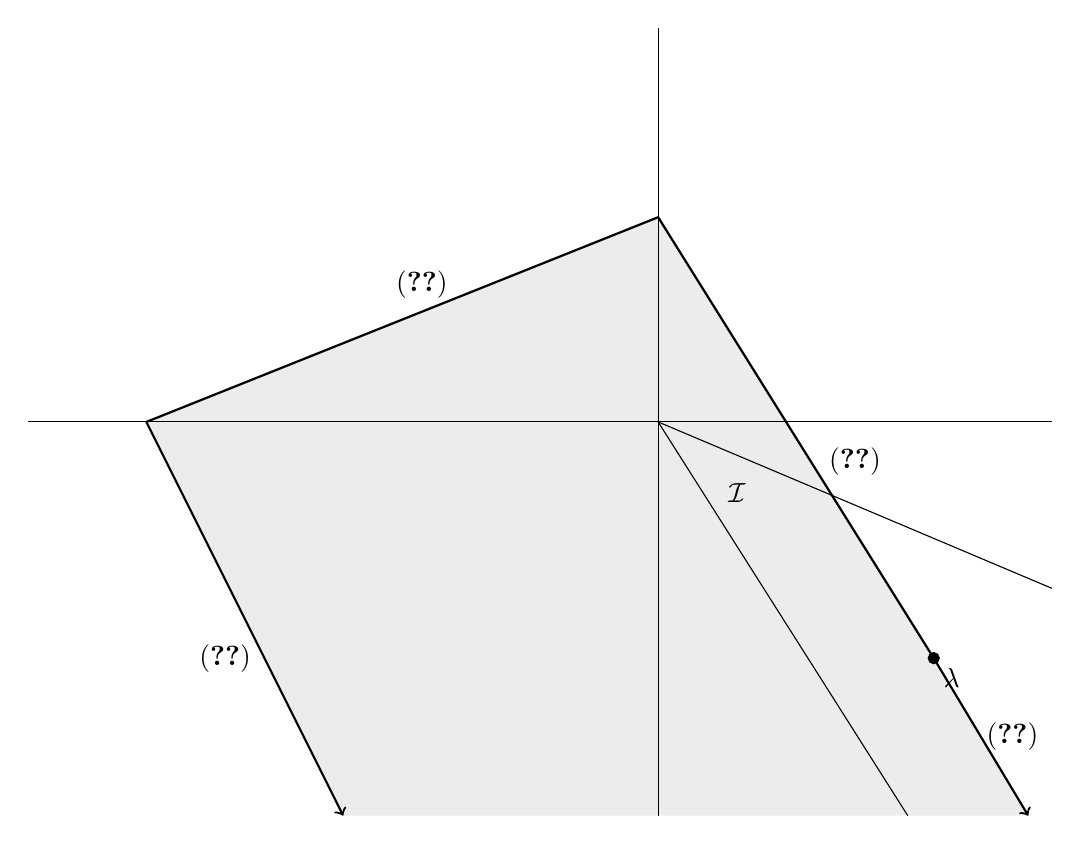
\begin{tikzpicture}
        \filldraw[color=lightgray!30] (47/10,-5) --(3.5,-3) -- (0,26/10) -- (-26/4,0) -- (-16/4,-5);
        \draw[-] (-8,0) -- (5,0);
        \draw[-] (0,-5) -- (0,5);
        %\filldraw[color=lightgray!30] (0,0) -- (5,-2.113) -- (5,-5) -- (3.17,-5) -- (0,0);
        \draw[-] (0,0) -- (5,-2.113);
        \draw[-] (0,0) -- (3.17,-5);
        \node at (1,-0.9) {$\cI$};
        \draw[fill=black] (3.5,-3) circle (2pt);
        \node[below right] at (3.5,-3) {$\lambda$};
        \draw[->,thick] (3.5,-3) -- (47/10,-5);
        \draw[-,thick] (3.5,-3) -- (0,26/10);
        \draw[-,thick] (0,26/10) -- (-26/4,0);
        \draw[->,thick] (-26/4,0) -- (-16/4,-5);
        \node at (4.5,-4) {\eqref{ineq:1}};
        \node at (2.5,-0.5) {\eqref{ineq:2}};
        \node at (-3,1.75) {\eqref{ineq:3}};
        \node at (-5.5,-3) {\eqref{ineq:4}};
      \end{tikzpicture}
    \]
  \end{lemma}
  \begin{proof}
    Following Lemma~\ref{le:imaginary transformations}, we consider even and odd sequences of mutations separately.

    For $i=2j$, $j>0$, and $\lambda\in\cI$, we observe that $\cC_{t_i}(\phi_{t_i}\lambda)\subset\RR^2$ is given by the inequalities 
    \[ (\dagger)\ x\le u_{2j+1,+}\lambda_1+u_{2j,+}\lambda_2 \qquad\text{and}\qquad (\ddagger)\ -y\le u_{2j,-}\lambda_1+u_{2j-1,-}\lambda_2. \]
    We inductively compute the region $\phi_{t_{2j}}^{-1}\cC_{t_{2j}}(\phi_{t_{2j}}\lambda)$, using Lemma~\ref{le:transformed inequalities} and the equality $\phi_{t_{2j}}^{-1}=\phi_{t_2}^{-j}$.

    \subsubsection*{Claim:} For $k>0$, $\phi_{t_{2k}}^{-1}\cC_{t_{2j}}(\phi_{t_{2j}}\lambda)$ is the region determined by the inequalities 
    \begin{align*}
      \tag{a} u_{2k,-}x+u_{2k-1,+}y &\le u_{2j,-}\lambda_1+u_{2j-1,+}\lambda_2;\\
      \tag{b} u_{2k+1,-}x+u_{2k,+}y &\le u_{2j+1,-}\lambda_1+u_{2j,+}\lambda_2;\\
      \tag{c} -u_{2k-1,-}x+u_{2k,+}y &\le u_{2j+1,-}\lambda_1+u_{2j,+}\lambda_2;\\
      \tag{d} -u_{2k-1,-}x-u_{2k-2,+}y &\le u_{2j+1,-}\lambda_1+u_{2j,+}\lambda_2.
    \end{align*}

    We see from \eqref{eq:backward two step mutation}, that $\lambda\in\cI$ implies the boundary ray for $\cC_{t_{2j}}(\phi_{t_{2j}}\lambda)$ corresponding to ($\ddagger$) lies entirely in the region in which $\phi_{t_2}^{-1}$ acts according to the matrix $\left[ \begin{array}{cc} -1 & -b\\ c & bc-1 \end{array}\right]$ of determinant 1.
    By Lemma~\ref{le:transformed inequalities}, the inequality ($\ddagger$) transforms into the inequality $cx+y\le u_{i,-}\lambda_1+u_{i-1,+}\lambda_2$ which corresponds to (a) with $k=1$.
    Similarly, the boundary ray for $\cC_{t_{2j}}(\phi_{t_{2j}}\lambda)$ corresponding to ($\dagger$) intersects three domains of linearity in which $\phi_{t_2}^{-1}$ acts according to the matrices $\left[ \begin{array}{cc} -1 & -b\\ c & bc-1 \end{array}\right]$, $\left[ \begin{array}{cc} -1 & -b\\ 0 & -1 \end{array}\right]$, $\left[ \begin{array}{cc} -1 & 0\\ 0 & -1 \end{array}\right]$, each of determinant 1.
    By Lemma~\ref{le:transformed inequalities}, the inequality ($\dagger$) can be seen to transform by these into each of inequalities (b), (c), (d) with $k=1$.
    This establishes the base of an induction on $k$.

    Assuming the inequalities (a)-(d) hold for $k$, we apply Lemma~\ref{le:transformed inequalities} with $\phi_{t_2}^{-1}$.
    Both of the boundary rays corresponding to the inequalities (a) and (d) lies entirely in the region where $\phi_{t_2}^{-1}$ acts according to the matrix $\left[ \begin{array}{cc} -1 & -b\\ c & bc-1 \end{array}\right]$, also the boundary segment corresponding to (b) intersects this region.
    Thus applying Lemma~\ref{le:transformed inequalities} to (a) gives the inequality 
    \[u_{2k+2,-}x+u_{2k+1,+}y=(u_{3,+}u_{2k,-}-u_{2,-}u_{2k-1,+})x+(u_{2,+}u_{2k,-}-u_{1,-}u_{2k-1,+})y\le u_{2j,-}\lambda_1+u_{2j-1,+}\lambda_2,\]
    which is the inequality (a) for $k+1$ by Lemma~\ref{eq:long Chebyshev recursion}; while applying this to (d) gives the inequality 
    \[-u_{2k+1,-}x-u_{2k,+}y=(-u_{3,+}u_{2k-1,-}+u_{2,-}u_{2k-2,+})x+(-u_{2,+}u_{2k-1,-}+u_{1,-}u_{2k-2,+})y\le u_{2j+1,-}\lambda_1+u_{2j,+}\lambda_2,\]
    which is the inequality (d) for $k+1$ again by Lemma~\ref{eq:long Chebyshev recursion}; finally applying this to (b) gives the inequality 
    \[u_{2k+3,-}x+u_{2k+2,+}y=(u_{3,+}u_{2k+1,-}-u_{2,-}u_{2k,+})x+(u_{2,+}u_{2k+1,-}-u_{1,-}u_{2k,+})y\le u_{2j+1,-}\lambda_1+u_{2j,+}\lambda_2,\]
    which is the inequality (b) for $k+1$.
    Similarly, the boundary segment corresponding to (c) lies entirely in the region where $\phi_{t_2}^{-1}$ acts according to the matrix $\left[ \begin{array}{cc} -1 & 0\\ c & -1 \end{array}\right]$.
    Thus applying Lemma~\ref{le:transformed inequalities} to (c) gives the inequality 
    \[-u_{2k+1,-}x-u_{2k,+}y=(u_{1,+}u_{2k-1,-}-u_{2,-}u_{2k,+})x+(-u_{0,+}u_{2k-1,-}-u_{1,-}u_{2k,+})y\le u_{2j+1,-}\lambda_1+u_{2j,+}\lambda_2,\]
    which is the inequality (d) for $k+1$ by Lemma~\ref{eq:long Chebyshev recursion}, in particular we see that the segment determined by (c) and the ray determined by (d) align in the image.
    Lastly, the boundary segment corresponding to (b) also intersects the regions where $\phi_{t_2}^{-1}$ acts according to the matrices $\left[ \begin{array}{cc} -1 & -b\\ 0 & -1 \end{array}\right]$ and $\left[ \begin{array}{cc} -1 & 0\\ 0 & -1 \end{array}\right]$ respectively.
    Applying Lemma~\ref{le:transformed inequalities} to (b) with the first matrix gives the inequality 
    \[-u_{2k+1,-}x+u_{2k+2,+}y=(-u_{1,+}u_{2k+1,-}+u_{0,-}u_{2k,+})x+(u_{2,+}u_{2k+1,-}-u_{1,-}u_{2k,+})y\le u_{2j+1,-}\lambda_1+u_{2j,+}\lambda_2,\]
    which is the inequality (c) for $k+1$ by Lemma~\ref{eq:long Chebyshev recursion}, while applying Lemma~\ref{le:transformed inequalities} to (b) with the second matrix gives the inequality 
    \[-u_{2k+1,-}x-u_{2k,+}y\le u_{2j+1,-}\lambda_1+u_{2j,+}\lambda_2,\]
    which again reproduces the inequality (d) and aligns with the previous segment and ray in the image.
    This completes the induction on $k$, proving the Claim and the result for $i$ even.

    For $i=2j+1$, $j>0$, and $\lambda\in\cI$, we get $\cC_{t_{2j+1}}(\phi_{t_{2j+1}}\lambda)\subset\RR^2$ is given by the inequalities 
    \[ (\dagger')\ -x\le u_{2j+1,+}\lambda_1+u_{2j,+}\lambda_2 \qquad\text{and}\qquad (\ddagger')\ y\le u_{2j+2,-}\lambda_1+u_{2j+1,-}\lambda_2.\]
    Using that $\phi_{t_{2j+1}}^{-1}=\phi_{t_2}^{-j}\phi_{t_1}^{-1}$, we compute the image inductively as above.
    From \eqref{eq:forward mutation 1} and Lemma~\ref{le:imaginary stability}, we see that the boundary ray for $\cC_{t_{2j+1}}(\phi_{t_{2j+1}}\lambda)$ corresponding to ($\dagger'$) lies entirely in the region in which $\phi_{t_1}^{-1}$ acts according to the matrix $\left[ \begin{array}{cc} -1 & 0\\ c & 1 \end{array}\right]$ of determinant $-1$.
    Thus applying Lemma~\ref{le:transformed inequalities}, the inequality ($\dagger'$) is transformed by $\phi_{t_1}^{-1}$ into the inequality $x\le u_{2j+1,+}\lambda_1+u_{2j,+}\lambda_2$.
    The boundary ray corresponding to ($\ddagger'$) intersects both domains of linearity for $\phi_{t_1}^{-1}$ and thus produces the inequalities
    \[ cx+y\le u_{2j+2,+}\lambda_1+u_{2j+1,+}\lambda_2 \qquad\text{and}\qquad  y\le u_{2j+2,+}\lambda_1+u_{2j+1,+}\lambda_2.\]


    \subsubsection*{Claim:} For $k\ge 0$, $\phi_{t_{2k+1}}^{-1}\cC_{t_{2j+1}}(\phi_{t_{2j+1}}\lambda)$ is the region determined by the inequalities 
    \begin{align*}
      \tag{a$'$} u_{2k+1,-}x+u_{2k,+}y &\le u_{2j+1,-}\lambda_1+u_{2j,+}\lambda_2;\\
      \tag{b$'$} u_{2k+2,-}x+u_{2k+1,+}y &\le u_{2j+2,-}\lambda_1+u_{2j+1,+}\lambda_2;\\
      \tag{c$'$} -u_{2k,-}x+u_{2k+1,+}y &\le u_{2j+2,-}\lambda_1+u_{2j+1,+}\lambda_2;\\
      \tag{d$'$} -u_{2k,-}x-u_{2k-1,+}y &\le u_{2j+2,-}\lambda_1+u_{2j+1,+}\lambda_2.
    \end{align*}
    By essentially the same calculations as above, these inequalities reproduce under the action of $\phi_{t_2}^{-1}$ and this completes the proof.
  \end{proof}

  The standard Chebyshev polynomials (of the second kind) are defined by the recursion $u_{i+1}=ru_i-u_{i-1}$, $u_1=1$, $u_0=0$, which can be computed explicitly as
  \[u_i(r)=\frac{1}{2^i\sqrt{r^2-4}}\left(\big(r+\sqrt{r^2-4}\big)^i-\big(r-\sqrt{r^2-4}\big)^i\right).\]
  By the equalities 
  \[u_{i,\varepsilon}=\begin{cases} \frac{\sqrt{b}}{\sqrt{c}}u_i(\sqrt{bc}) & \text{if $i$ is even and $\varepsilon=+$;}\\ \frac{\sqrt{c}}{\sqrt{b}}u_i(\sqrt{bc}) & \text{if $i$ is even and $\varepsilon=-$;}\\ u_i(\sqrt{bc}) & \text{if $i$ is odd;} \end{cases}\]
  it follows that $u_{i,\varepsilon}$ can be computed explicitly as
  \[u_{i,\varepsilon}=\begin{cases} \frac{\sqrt{b}}{2^i\sqrt{c(bc-4)}}\left(\big(\sqrt{bc}+\sqrt{bc-4}\big)^i-\big(\sqrt{bc}-\sqrt{bc-4}\big)^i\right) & \text{if $i$ is even and $\varepsilon=+$;}\\ \frac{\sqrt{c}}{2^i\sqrt{b(bc-4)}}\left(\big(\sqrt{bc}+\sqrt{bc-4}\big)^i-\big(\sqrt{bc}-\sqrt{bc-4}\big)^i\right) & \text{if $i$ is even and $\varepsilon=-$;}\\ \frac{1}{2^i\sqrt{bc-4}}\left(\big(\sqrt{bc}+\sqrt{bc-4}\big)^i-\big(\sqrt{bc}-\sqrt{bc-4}\big)^i\right) & \text{if $i$ is odd.} \end{cases}\]
  \begin{remark}
    Note that $u_{2j+1,+}=u_{2j+1,-}$ for all $j\in\ZZ$.
    Moreover, since $u_{-i,\varepsilon}=-u_{i,\varepsilon}$, these formulas can also easily be seen to hold for $i<0$.
  \end{remark}

  \begin{lemma}
    We have
    \[\lim_{i\to\infty} \frac{-u_{i,-}}{u_{i-1,+}}=\frac{-bc-\sqrt{bc(bc-4)}}{2b} \qquad \lim_{i\to\infty} \frac{-u_{i-1,-}}{u_{i,+}}=\frac{-bc+\sqrt{bc(bc-4)}}{2b}.\]
  \end{lemma}
  \begin{proof}
    For any $i\ge 1$, we have
    \[\frac{\big(\sqrt{bc}+\sqrt{bc-4}\big)^i-\big(\sqrt{bc}-\sqrt{bc-4}\big)^i}{\big(\sqrt{bc}+\sqrt{bc-4}\big)^{i-1}-\big(\sqrt{bc}-\sqrt{bc-4}\big)^{i-1}}=\frac{\sqrt{bc}+\sqrt{bc-4}}{1-\left(\frac{\sqrt{bc}-\sqrt{bc-4}}{\sqrt{bc}+\sqrt{bc-4}}\right)^{i-1}}.\]
    It follows that
    \[\lim_{i\to\infty} \frac{-u_{i,-}}{u_{i-1,+}} = \lim_{i\to\infty} \left( \frac{-\sqrt{c}}{2\sqrt{b}}\cdot\frac{\sqrt{bc}+\sqrt{bc-4}}{1-\left(\frac{\sqrt{bc}-\sqrt{bc-4}}{\sqrt{bc}+\sqrt{bc-4}}\right)^{i-1}} \right) = \frac{-\sqrt{c}}{2\sqrt{b}}\cdot\big(\sqrt{bc}+\sqrt{bc-4}\big),\]
    which is equivalent to the desired expression.
    Similarly, 
    \[\frac{\big(\sqrt{bc}+\sqrt{bc-4}\big)^{i-1}-\big(\sqrt{bc}-\sqrt{bc-4}\big)^{i-1}}{\big(\sqrt{bc}+\sqrt{bc-4}\big)^i-\big(\sqrt{bc}-\sqrt{bc-4}\big)^i}=\frac{\sqrt{bc}-\sqrt{bc-4}}{4\left(1-\left(\frac{\sqrt{bc}-\sqrt{bc-4}}{\sqrt{bc}+\sqrt{bc-4}}\right)^i\right)},\]
    so that
    \[\lim_{i\to\infty} \frac{-u_{i-1,-}}{u_{i,+}} = \lim_{i\to\infty} \left( \frac{-2\sqrt{c}}{\sqrt{b}}\cdot\frac{\sqrt{bc}-\sqrt{bc-4}}{4\left(1-\left(\frac{\sqrt{bc}-\sqrt{bc-4}}{\sqrt{bc}+\sqrt{bc-4}}\right)^{i-1}\right)} \right) = \frac{-\sqrt{c}}{2\sqrt{b}}\cdot\big(\sqrt{bc}-\sqrt{bc-4}\big),\]
    which is again equivalent to the desired expression.
  \end{proof}

  \begin{lemma}
    If $\lambda\in\ZZ^2\setminus\cI$, then $\cP(\lambda)=\{\lambda\}$.
  \end{lemma}
  \begin{proof}
    It is enough to consider $\phi_{t_{-2}}^{-1}\cC(\phi_{t_{-2}}\lambda) \cap \cC(\lambda) \cap \phi_{t_2}^{-1}\cC(\phi_{t_2}\lambda)$, we leave the details to the reader.
  \end{proof}

  \begin{lemma}
    \label{le:one direction}
    For $\lambda\in\cI\cap\ZZ^2$, 
    \begin{enumerate}
      \item $\cP_+(\lambda):=\bigcap_{i \ge 0}\phi_{t_i}^{-1}\cC(\phi_{t_i}\lambda)$ is the quadrilateral with corner vertices $\lambda$, $(\frac{2-bc-\sqrt{bc(bc-4)}}{2}\lambda_1-\frac{bc+\sqrt{bc(bc-4)}}{2c}\lambda_2,0)$, $(0,\frac{bc+\sqrt{bc(bc-4)}}{2b}\lambda_1+\lambda_2)$, and $(\frac{2-bc-\sqrt{bc(bc-4)}}{2}\lambda_1-b\lambda_2,\lambda_2)$.
      \item $\cP_-(\lambda):=\bigcap_{i \le 0}\phi_{t_i}^{-1}\cC(\phi_{t_i}\lambda)$ is the quadrilateral with corner vertices $\lambda$, $(\lambda_1+\frac{bc+\sqrt{bc(bc-4)}}{2c}\lambda_2,0)$, $(0,-\frac{bc+\sqrt{bc(bc-4)}}{2b}\lambda_1+\frac{2-bc-\sqrt{bc(bc-4)}}{2}\lambda_2)$, and $(\lambda_1,-c\lambda_1+\frac{2-bc-\sqrt{bc(bc-4)}}{2}\lambda_2)$.
    \end{enumerate}
  \end{lemma}
  \begin{proof}
    We prove (1) as (2) is obtained by interchanging $b$ with $c$ and swapping all ordered pairs.  
    We first show that $\cC(\lambda) \cap \phi_{t_i}^{-1}\cC(\phi_{t_i}\lambda)\supsetneq \cC(\lambda) \cap \phi_{t_j}^{-1}\cC(\phi_{t_j}\lambda)$ for $0\le i<j$.
  \end{proof}

  \begin{theorem}
    For $\lambda\in\cI\cap\ZZ^2$, there are five classes of dominance polytopes.
    \begin{enumerate}
      \item if $\lambda$ lies in the interior of the cone spanned by the vectors $(2b,-bc-\sqrt{bc(bc-4)})$ and $(2,-c)$, then $\cC(\lambda)$ is the trapezoid with corner vertices $\lambda$, $(\frac{2-bc-\sqrt{bc(bc-4)}}{2}\lambda_1-\frac{bc+\sqrt{bc(bc-4)}}{2c}\lambda_2,0)$, $(0,\frac{bc+\sqrt{bc(bc-4)}}{2b}\lambda_1+\lambda_2)$, and ???.
      \item if $\lambda$ lies on the ray spanned by $(2,-c)$, say $\lambda=(2\ell,-c\ell)$, then $\cC(\lambda)$ is the triangle with corner vertices $\lambda$, $(2\ell-\frac{bc+\sqrt{bc(bc-4)}}{2}\ell,0)$, and $(0,\frac{\sqrt{bc(bc-4)}}{b}\ell)$.
      \item if $\lambda$ lies in the interior of the cone spanned by the vectors $(2,-c)$ and $(b,-2)$, then $\cC(\lambda)$ is the kite with corner vertices $\lambda$, $(\lambda_1+\frac{bc+\sqrt{bc(bc-4)}}{2c}\lambda_2,0)$, $\frac{bc+\sqrt{bc(bc-4)}}{2\sqrt{bc(bc-4)}}(2\lambda_1+b\lambda_2,c\lambda_1+2\lambda_2)$, and $(0,\frac{bc+\sqrt{bc(bc-4)}}{2b}\lambda_1+\lambda_2)$.
      \item if $\lambda$ lies on the ray spanned by $(b,-2)$, say $\lambda=(b\ell,-2\ell)$, then $\cC(\lambda)$ is the triangle with corner vertices $\lambda$, $(-\frac{\sqrt{bc(bc-4)}}{c}\ell,0)$, and $(0,\frac{bc+\sqrt{bc(bc-4)}}{2}\ell-2\ell)$.
      \item if $\lambda$ lies in the interior of the cone spanned by the vectors $(b,-2)$ and $(2b,-bc+\sqrt{bc(bc-4)})$, then $\cC(\lambda)$ is the triangle with corner vertices $\lambda$, $(\lambda_1+\frac{bc+\sqrt{bc(bc-4)}}{2c}\lambda_2,0)$, $(0,-\frac{bc+\sqrt{bc(bc-4)}}{2b}\lambda_1+\frac{2-bc-\sqrt{bc(bc-4)}}{2}\lambda_2)$, and ???.
    \end{enumerate}
  \end{theorem}
  \begin{proof}
    Following Lemma~\ref{le:one direction}, we see that the intersection $\cP_+(\lambda)\cap\cP_-(\lambda)$ degenerates to a triangle precisely when
    \[\frac{2-bc-\sqrt{bc(bc-4)}}{2}\lambda_1-\frac{bc+\sqrt{bc(bc-4)}}{2c}\lambda_2=\lambda_1+\frac{bc+\sqrt{bc(bc-4)}}{2c}\lambda_2\]
    or 
    \[\frac{bc+\sqrt{bc(bc-4)}}{2b}\lambda_1+\lambda_2=-\frac{bc+\sqrt{bc(bc-4)}}{2b}\lambda_1+\frac{2-bc-\sqrt{bc(bc-4)}}{2}\lambda_2.\]
    The first equations reduces to $c\lambda_1+2\lambda_2=0$, while the second reduces to $2\lambda_1+b\lambda_2=0$.
    In particular, the rays spanned by $(2,-c)$ and $(b,-2)$ determine this change of state in the dominance regions $\cP(\lambda)$.
  \end{proof}

  \begin{remark}
    Note that the rays which separate the regions inside $\cI$ correspond exactly to the columns of the associated Cartan matrix $\left[ \begin{array}{cc} 2 & -b \\ -c & 2 \end{array} \right]$.
    This unexpected coincidence is one of our reasons for deciding to write down these results.
  \end{remark}

  The dominance polygon pointed at $\lambda=(\lambda_1,\lambda_2)$ is the region defined by the following six inequalities:
  \begin{align}
    -\lambda_1-\frac{b c+\sqrt{b c (b c-4)}}{2 c}\lambda_2+x+\frac{b c+\sqrt{b c (b c-4)}}{2 c}y\geq0
    \\
    \frac{b c+\sqrt{b c (b c-4)}}{2 b}\lambda_1+\lambda_2-\frac{b c+\sqrt{b c (b c-4)}}{2 b}x-y\geq0
    \\
    -\frac{b c+\sqrt{b c (b c-4)}}{2 b}\lambda_1 - \frac{b c+\sqrt{b c (b c-4)}-2}{2}\lambda_2 + \frac{b c+\sqrt{b c (b c-4)}}{2 b}x-y\geq0
    \\
    \frac{b c+\sqrt{b c (b c-4)}-2}{2}\lambda_1+\frac{b c+\sqrt{b c (b c-4)}}{2 c}\lambda_2+x-\frac{b c+\sqrt{b c (b c-4)}}{2 c}y\geq0
    \\
    -\frac{b c+\sqrt{b c (b c-4)}}{2 b}\lambda_1-\frac{b c+\sqrt{b c (b c-4)}-2}{2}\lambda_2-\frac{b c-\sqrt{b c (b c-4)}}{2 b}x-y\geq0
    \\
    \frac{b c+\sqrt{b c (b c-4)}-2}{2}\lambda_1+\frac{b c+\sqrt{b c (b c-4)}}{2 c}\lambda_2+x+\frac{b c-\sqrt{b c (b c-4)}}{2 c}y\geq0
  \end{align}
  Are any of these better forms?
  \begin{align}
    (x-\lambda_1)+\frac{b c+\sqrt{b c (b c-4)}}{2 c}(y-\lambda_2)\geq0
    \\
    \nonumber \iff \frac{b c-\sqrt{b c (b c-4)}}{2 b}(x-\lambda_1)+(y-\lambda_2)\geq0
    \\
    -\frac{b c+\sqrt{b c (b c-4)}}{2 b}(x-\lambda_1)-(y-\lambda_2)\geq0
    \\
    \nonumber \iff -(x-\lambda_1)-\frac{b c-\sqrt{b c (b c-4)}}{2 c}(y-\lambda_2)\geq0
    \\
    -\frac{b c+\sqrt{b c (b c-4)}}{2}\lambda_2 + \frac{b c+\sqrt{b c (b c-4)}}{2 b}(x-\lambda_1)-(y-\lambda_2)\geq0
    \\
    \nonumber \iff -b\lambda_2 + (x-\lambda_1)-\frac{b c-\sqrt{b c (b c-4)}}{2 c}(y-\lambda_2)\geq0
    \\
    \frac{b c+\sqrt{b c (b c-4)}}{2}\lambda_1+(x-\lambda_1)-\frac{b c+\sqrt{b c (b c-4)}}{2 c}(y-\lambda_2)\geq0
    \\
    \nonumber \iff c\lambda_1+\frac{b c-\sqrt{b c (b c-4)}}{2 b}(x-\lambda_1)-(y-\lambda_2)\geq0
    \\
    -c\lambda_1-\frac{b c+\sqrt{b c (b c-4)}}{2}\lambda_2-\frac{b c-\sqrt{b c (b c-4)}}{2 b}(x-\lambda_1)-(y-\lambda_2)\geq0
    \\
    \frac{b c+\sqrt{b c (b c-4)}}{2}\lambda_1+b\lambda_2+(x-\lambda_1)+\frac{b c-\sqrt{b c (b c-4)}}{2 c}(y-\lambda_2)\geq0
  \end{align}
  Another proposal (I also changed the order of the equations)
  \begin{align}
    \frac{b c-\sqrt{b c (b c-4)}}{2 b}(x-\lambda_1)+(y-\lambda_2) & \geq0
    \\
    \frac{b c+\sqrt{b c (b c-4)}}{2 b}(x-\lambda_1-b\lambda_2)-(y-\lambda_2) & \geq 0
    \\
    -\frac{b c-\sqrt{b c (b c-4)}}{2 b}(x-\lambda_1)-(y-\lambda_2)& \geq c\lambda_1+\frac{b c+\sqrt{b c (b c-4)}}{2b}b\lambda_2
    \\
    -(x-\lambda_1)-\frac{b c-\sqrt{b c (b c-4)}}{2 c}(y-\lambda_2)& \geq0
    \\
    (x-\lambda_1)-\frac{b c+\sqrt{b c (b c-4)}}{2 c}(y-\lambda_2-c\lambda_1) & \geq 0
    \\
    (x-\lambda_1)+\frac{b c-\sqrt{b c (b c-4)}}{2 c}(y-\lambda_2) & \geq -\frac{b c+\sqrt{b c (b c-4)}}{2c}c\lambda_1-b\lambda_2
  \end{align}
  Maybe this one:
  \begin{align}
    \frac{b c-\sqrt{b c (b c-4)}}{2 b}(x-\lambda_1)+(y-\lambda_2) & \geq0
    \\
    \frac{b c+\sqrt{b c (b c-4)}}{2 b}(x-\lambda_1-b\lambda_2)-(y-\lambda_2) & \geq 0
    \\
    -\frac{b c-\sqrt{b c (b c-4)}}{2 b}(x-\lambda_1)-(y-\lambda_2)& \geq c\lambda_1+\frac{b c+\sqrt{b c (b c-4)}}{2b}b\lambda_2
    \\
    -(x-\lambda_1)-\frac{b c-\sqrt{b c (b c-4)}}{2 c}(y-\lambda_2)& \geq0
    \\
    (x-\lambda_1)-\frac{b c+\sqrt{b c (b c-4)}}{2 c}(y-\lambda_2-c\lambda_1) & \geq 0
    \\
    (x-\lambda_1)+\frac{b c-\sqrt{b c (b c-4)}}{2 c}(y-\lambda_2) & \geq -\frac{b c+\sqrt{b c (b c-4)}}{2c}c\lambda_1-b\lambda_2
  \end{align}

  Yet another version:
 
 {
    \everymath={\displaystyle}
  \[
  \begin{array}{rcccl}
    -c\lambda_1-\frac{b c+\sqrt{b c (b c-4)}}{2b}b\lambda_2 & \geq & \frac{b c-\sqrt{b c (b c-4)}}{2 b}(x-\lambda_1)+(y-\lambda_2) & \geq & 0
    \\
    &  & \frac{b c-\sqrt{b c (b c-4)}}{2 b}(x-\lambda_1)-(y-\lambda_2) & \geq & c\lambda_1
    \\
    - b \lambda_2 & \geq & - (x-\lambda_1) + \frac{b c-\sqrt{b c (b c-4)}}{2 c} (y-\lambda_2) 
    \\
    0 & \geq & (x-\lambda_1)+\frac{b c-\sqrt{b c (b c-4)}}{2 c}(y-\lambda_2) & \geq &-\frac{b c+\sqrt{b c (b c-4)}}{2c}c\lambda_1-b\lambda_2
  \end{array}
\]
}

Or: (Maybe at this point we can remove $c/c$ and $b/b$)

 {
    \everymath={\displaystyle}
  \[
  \begin{array}{rcccl}
    -c\lambda_1-\frac{b c+\sqrt{b c (b c-4)}}{2b}b\lambda_2 & \geq & \frac{b c-\sqrt{b c (b c-4)}}{2 b}(x-\lambda_1)+(y-\lambda_2) & \geq & 0
    \\
    &  & \frac{b c-\sqrt{b c (b c-4)}}{2 b}(x-\lambda_1)-(y-\lambda_2) & \geq & c\lambda_1
    \\
    -\frac{b c+\sqrt{b c (b c-4)}}{2c}c\lambda_1-b\lambda_2  & \leq & (x-\lambda_1)+\frac{b c-\sqrt{b c (b c-4)}}{2 c}(y-\lambda_2) & \leq & 0
    \\
    & & - (x-\lambda_1) + \frac{b c-\sqrt{b c (b c-4)}}{2 c} (y-\lambda_2)  & \leq & - b \lambda_2
  \end{array}
\]
}


  \subsection{Deformation Support}
  The greedy basis of Lee, Li, and Zelevinsky \cite{lee-li-zelevinsky} can be defined as the positive pointed basis with minimal support.
  Here we identify the maximum possible support of its deformations.

  It will be convenient later to have explicit expressions for the greedy basis elements so we recall here the combinatorial construction of their Laurent expansions.
  For a $\bfg$-vector $\lambda\in\ZZ^2\setminus\ZZ_{\ge0}^2$, define the \emph{maximal Dyck path} $D_\lambda\subset\ZZ^2$ to be the lattice path with corner vertices $(0,0)$ and $(a_1,a_2):=\big([-\lambda_1+b\lambda_2]_+,[-\lambda_2]_+\big)$ which is maximal in the following sense:
  \begin{itemize}
    \item every lattice point of $D_\lambda$ lies below the line connecting the corner vertices;
    \item any lattice point above $D_\lambda$ lies above the line connecting the corner vertices.
  \end{itemize}
  For $\lambda\in\ZZ_{\ge0}^2$, we take $D_\lambda$ to be the empty path at $(0,0)$.

  We consider $D_\lambda$ to be the set of its edges ordered from $(0,0)$.
  Write $H_\lambda,V_\lambda\subset D_\lambda$ for the subsets of horizontal and vertical edges, respectively.
  According to the ordering of $D_\lambda$, we denote $H_\lambda=\{h_1,\ldots,h_{a_1}\}$ and $V_\lambda=\{v_1,\ldots,v_{a_2}\}$.
  For edges $e,e'\in D_\lambda$ with $e\le e'$, write $ee'\subset D_\lambda$ for the shortest subpath of $D_\lambda$ containing $e$ and $e'$.
  For edges $e,e'\in D_\lambda$ with $e'<e$, write $ee'\subset D_\lambda$ for the subset $ev_{a_2} \sqcup h_1e'$, which can be seen as the subpath traversing from the edge $e$ to the end of $D_\lambda$ and then continuing from the beginning of $D_\lambda$ to the edge $e'$.
  For any subset $S\subset D_\lambda$, write $|S|_H:=|S\cap H_\lambda|$ and $|S|_V:=|S\cap V_\lambda|$; in particular, for $e,e'\in D_\lambda$, write $|ee'|_H:=|ee'\cap H_\lambda|$ and $|ee'|_V:=|ee'\cap V_\lambda|$.
  \begin{definition}
    A subset $S\subset D_\lambda$ is said to be \emph{compatible} if: for every $h\in S\cap H_\lambda$ and $v\in S\cap V_\lambda$, there exists an edge $e\in hv$ so that one of the following conditions is satisfied:
    \begin{align*}
      e\ne v \quad \text{and} \quad |he|_V=c|he\cap S|_H;\\
      e\ne h \quad \text{and} \quad |ev|_H=b|ev\cap S|_V.
    \end{align*}
    Write $\cC_\lambda$ for the set of all compatible subsets $S\subset D_\lambda$.
  \end{definition}

  The \emph{greedy basis element} $x^{gr}_\lambda$ is then given by the following Laurent polynomial
  \begin{equation}
    \label{eq:greedy}
    x^{gr}_\lambda=x_1^{\lambda_1}x_2^{\lambda_2} \sum_{S\in \cC_\lambda} x_1^{b(|V_\lambda|-|S|_V)} x_2^{c|S|_H}.
  \end{equation}

  Consider the deformation of the theta basis element with $\bfg$-vector $\lambda$.
  \begin{theorem}
    For $\lambda\in\cI\cap\ZZ^2$, the support of any deformation of the corresponding theta basis element is contained in the polytope defined by the following inequalities:
    \begin{align*}
       \lambda_1-b\lambda_2 &\le x\\
       \lambda_2 &\le y\\
    \end{align*}
    is the convex hull of the following vertices:
    \[\lambda, \qquad (\lambda_1-b\lambda_2,\lambda_2), \qquad (\lambda_1-b\lambda_2,\lambda_2-c\lambda_1), \qquad (?,?)\]
    The $d$-vector is $(\lambda_1-b\lambda_2,\lambda_2)$

    $\frac{bc+\sqrt{bc(bc-4)}}{2\sqrt{bc(bc-4)}}(2\lambda_1+b\lambda_2,c\lambda_1+2\lambda_2)$, and $(0,\frac{bc+\sqrt{bc(bc-4)}}{2b}\lambda_1+\lambda_2)$

    Slope:
    \[\big(\frac{bc+\sqrt{bc(bc-4)}}{2\sqrt{bc(bc-4)}}(c\lambda_1+2\lambda_2)-(\frac{bc+\sqrt{bc(bc-4)}}{2b}\lambda_1+\lambda_2)\big) /\frac{bc+\sqrt{bc(bc-4)}}{2\sqrt{bc(bc-4)}}(2\lambda_1+b\lambda_2)\]

    $y=$

    $(\lambda_1,\lambda_2)$ and $(0,\frac{bc+\sqrt{bc(bc-4)}}{2b}\lambda_1+\lambda_2)$
    
    Slope: $-\frac{bc+\sqrt{bc(bc-4)}}{2b}$\\

    Corner of dominant support?: 
    \begin{align*}
      \left(\frac{bc+\sqrt{bc(bc-4)}}{2\sqrt{bc(bc-4)}}(2\lambda_1+b\lambda_2),-\frac{bc+\sqrt{bc(bc-4)}}{2b}\frac{bc+\sqrt{bc(bc-4)}}{2\sqrt{bc(bc-4)}}(2\lambda_1+b\lambda_2)+\frac{bc+\sqrt{bc(bc-4)}}{2b}\lambda_1+\lambda_2\right)\\
      \left(\frac{bc+\sqrt{bc(bc-4)}}{2\sqrt{bc(bc-4)}}(2\lambda_1+b\lambda_2),-\frac{bc+\sqrt{bc(bc-4)}}{2b}\frac{bc}{\sqrt{bc(bc-4)}}\lambda_1+-\frac{bc+\sqrt{bc(bc-4)}}{2}\frac{bc+\sqrt{bc(bc-4)}}{2\sqrt{bc(bc-4)}}\lambda_2+\lambda_2\right)\\
    \end{align*}
    
  \end{theorem}


  \section{The Total Domination Polyhedron}

  Define the \emph{total domination polyhedron} $\cD:=\{(\lambda,\mu):\mu\in\cP(\lambda)\}$, i.e. this is the set of all pairs where $\lambda$ dominates $\mu$.
  Write $\pi_1:\cD\to\RR^n$ for the projection to $\lambda$ and $\pi_2:\cD\to\RR^n$ for the projection to $\mu$.
  \begin{itemize}
    \item Is it a polyhedron?
    \item The lemma below might suggest so.  
      Indeed, if it is, by the Decomposition Theorem, we can write $\cD$ as the Minkowski sum of a polyhedral cone (almost certainly $\cI$) and a convex polytope (what is it?).
      I am ignoring that it should really be the union of this polyhedron with a plane if the previous sentence holds any water.
    \item Actually, we might need to take the union of several polyhedra to account for the variations in the fibers $\pi_1^{-1}(\lambda)$.
  \end{itemize}

  Is the following result true beyond rank 2?
  \begin{lemma}
    For $\mu\in\RR^2$, $\pi_2^{-1}(\mu)$ is a translate of the imaginary cone $\cI$ or the union of such with a single point.
  \end{lemma}
  \begin{proof}
    For $\mu$ in the second quadrant, the vertex of this cone should be given by $\lambda=(\lambda_1,\lambda_2)$ where
    \[\lambda_1=\frac{2b\mu_2-4\mu_1}{bc-4+\sqrt{bc(bc-4)}} \qquad \text{and} \qquad \lambda_2=\frac{2c\mu_1-4\mu_2}{bc-4+\sqrt{bc(bc-4)}}.\]
    (This comes from setting $\mu$ to be the vertex opposite $\lambda$ inside the dominance region $\cP(\lambda)$ and then solving for $\lambda$.)
  \end{proof}
  \begin{remark}
    We want to understand what the curve is that results when we have $\mu$ lie along the unit circle, this should be possible by plugging $(\cos(\theta),\sin(\theta))$ into this formula for $\lambda$ and seeing what ellipse we get.
  \end{remark}


  \section{Bases From Compatible Pairs on Dyck Paths}
  \sayDR{This is a bit of a repetition of the above introduction to Dyck paths, but with slightly different goals it seemed that a modified exposition was more appropriate.}
  For $a_1,a_2\in\ZZ_{\ge0}$, choose a Dyck path $D$ in the lattice rectangle $[0,a_1]\times[0,a_2]$.
  When we wish to emphasize the upper right bounding corner we will write $D[a_1,a_2]$.
  Consider $D$ as the totally ordered set of its edges along the natural labeling from $(0,0)$ to $(a_1,a_2)$.
  It may be convenient to identify $D$ with the ordered set $[1,a_1+a_2]$.
  Write $D=D_1\sqcup D_2$, where $D_1=\{h_1,\ldots,h_{a_1}\}$ is the set of horizontal edges and $D_2=\{v_1,\ldots,v_{a_2}\}$ is the set of vertical edges.
  Define the \emph{height}, $\hgt(h)$ for $h\in D_1$, as one more than the number of $v\in D_2$ with $v<h$.
  Define the \emph{depth}, $\dpt(v)$ for $v\in D_2$, as the number of $h\in D_1$ with $h<v$.
  \begin{remark}
    The seemingly different conventions for computing height and depth provide uniformity later.
    Indeed, the vertical edges immediately following $h_d$ have depth $d$, while this convention allows the horizontal edges immediately preceding $v_\ell$ to similarly be said to have height $\ell$.
  \end{remark}

  Observe that the data of $D$ is just the data of a bipartition of a finite totally ordered set $D=D_1\sqcup D_2$.
  Given a Dyck path $D=D_1\sqcup D_2$ in the lattice rectangle $[0,a_1]\times[0,a_2]$, write $\bar{D}=\bar{D}_1 \sqcup \bar{D}_2$ for the Dyck path (under the identification with $[1,a_1+a_2]$) in the lattice rectangle $[0,a_2]\times[0,a_1]$ with $\bar{D}_1=a_1+a_2+1-D_2$ and $\bar{D}_2=a_1+a_2+1-D_1$.
  This operation can be visualized as transposing the Dyck path.

  Given any quantity or object $P$ whose definition depends on $b$ and $c$, write $\vv{P}$ for the same quantity or object defined with $b$ and $c$ interchanged.
  In particular, we have $\vv{u}_{m,\varepsilon}=u_{m,-\varepsilon}$ for any $m$ and any $\varepsilon=\pm1$.

  \subsection{Structure of Dyck Paths}

  Write $D^{max}=D^{max}[a_1,a_2]$ for the maximal Dyck path in the lattice rectangle $[0,a_1]\times[0,a_2]$, i.e. $D^{max}$ never crosses above the diagonal line joining $(0,0)$ to $(a_1,a_2)$ and any lattice point above $D^{max}$ also lies above the diagonal.
  Observe that $\bar{D}^{max}[a_1,a_2]=D^{max}[a_2,a_1]$.

  \begin{definition}
    Call a Dyck path $D$ 
    \begin{itemize}
      \item \emph{horizontally-adapted to $b$} if no vertical edge of $D$ is immediately preceded by more than $b$ horizontal edges;
      \item \emph{vertically-adapted to $c$} if no horizontal edge of $D$ is immediately followed by more than $c$ vertical edges.
    \end{itemize}
  \end{definition}

  \begin{definition}
    \label{def:Dyck path mutations}
    Given a Dyck path $D=D[a_1,a_2]$ which is vertically-adapted to $c$, define a Dyck path $\mu_{1,c}(D)$ inside the lattice rectangle $[0,ca_1-a_2]\times[0,a_1]$ by replacing each horizontal edge of $D$, together with the $r$ vertical edges which immediately follow it, by $c-r$ horizontal edges followed by a vertical edge.
    This provides a canonical identification of the horizontal edges of $D$ with the vertical edges of $\mu_{1,c}(D)$, this identification is again denoted by $\mu_{1,c}$.

    Given a Dyck path $D=D[a_1,a_2]$ which is horizontally-adapted to $b$, define a Dyck path $\mu_{2,b}(D)$ inside the lattice rectangle $[0,a_2]\times[0,ba_2-a_1]$ by replacing each vertical edge of $D$, together with the $r$ horizontal edges which immediately precede it, by a horizontal edge followed by $b-r$ vertical edges.
    This provides a canonical identification of the vertical edges of $D$ with the horizontal edges of $\mu_{2,b}(D)$, this identification is again denoted by $\mu_{2,b}$.
  \end{definition}
  \begin{remark}
    Observe that $\mu_{1,a}$ and $\mu_{2,a}$ are inverse for any $a\ge1$ whenever they are defined.
  \end{remark}

  The following result is proven in \cite[Lemma 2.4]{rupel} with appropriate notation changes, c.f. Theorem~\ref{th:dominant Dyck path recursion} for a slight modification and explicit proof.
  \begin{lemma}\mbox{}
    \label{le:maximal Dyck path recursion}
    \begin{enumerate}
      \item If $a_2 < c a_1$, then $\mu_{1,c}\big(D^{max}[a_1,a_2]\big)=D^{max}[ca_1-a_2,a_1]$.
      \item If $a_1 < b a_2$, then $\mu_{2,b}\big(D^{max}[a_1,a_2]\big)=D^{max}[a_2,ba_2-a_1]$.
    \end{enumerate}
  \end{lemma}

  As an immediate consequence, we determine the structure of certain maximal Dyck paths.
  We introduce the following notation for convenience:
  \[d_m:=\begin{cases} b & \text{if $m$ is even;}\\ c & \text{if $m$ is odd;}\end{cases} \qquad \text{and} \qquad \vv{d}_m:=\begin{cases} c & \text{if $m$ is even;}\\ b & \text{if $m$ is odd;}\end{cases}\]
  The following was proven in \cite[Corollary 2.6]{rupel} and follows by a simple induction using Lemma~\ref{le:maximal Dyck path recursion}.
  \begin{corollary}
    Assume $b,c\ge2$ (this can be dropped with extra notation and slight modification).
    Then, for $\varepsilon=\pm1$ and $m\ge1$, the maximal Dyck path $D^{m,\varepsilon}:=D^{max}[u_{m,\varepsilon},u_{m-1,-\varepsilon}]$ can be constructed as follows:
    \begin{itemize}
      \item $D^{1,\varepsilon}$ consists of a single horizontal edge;
      \item $D^{2,\varepsilon}$ consists of $d_2$ horizontal edges followed by a vertical edge;
      \item for $m\ge3$, $D_{m,\varepsilon}$ consists of $d_m - 1$ copies of $D^{m-1,\varepsilon}$ followed by a copy of $D^{m-1,\varepsilon}$ with its first $D^{m-2,\varepsilon}$ removed;
    \end{itemize}
    and the maximal Dyck path $\vv{\bar{D}}^{m,\varepsilon}:=D^{max}[u_{m-1,\varepsilon},u_{m,-\varepsilon}]$ can be constructed as follows:
    \begin{itemize}
      \item $\vv{\bar{D}}^{1,\varepsilon}$ consists of a single vertical edge;
      \item $\vv{\bar{D}}^{2,\varepsilon}$ consists of a horizontal edge followed by $\vv{d}_2$ vertical edges;
      \item for $m\ge3$, $\vv{\bar{D}}^{m,\varepsilon}$ consists of a copy of $\vv{\bar{D}}^{m-1,\varepsilon}$ with its last $\vv{\bar{D}}^{m-2,\varepsilon}$ removed followed by $\vv{d}_m - 1$ copies of $\vv{\bar{D}}^{m-1,\varepsilon}$.
    \end{itemize}
  \end{corollary}

  Our main interest will be with the following Dyck paths.
  \begin{definition}
    \label{def:dominant Dyck path}
    For $a_1,a_2\in\ZZ_{\ge0}$ with $(-a_1+ba_2,-a_2)\in\cI$, define the \emph{dominant Dyck path} $D^{dom}=D^{dom}[a_1,a_2]$ to be the maximal Dyck path starting from $(0,0)$ and terminating at $(a_1,a_2)$ while staying below the lines $y=\frac{bc+\sqrt{bc(bc-4)}}{2b}x$ and $y-a_2=\frac{bc-\sqrt{bc(bc-4)}}{2b}(x-a_1)$.

    For $a_1,a_2\in\ZZ_{\ge0}$ with $(-a_2,-a_1+ca_2)\in\cI'$, define the \emph{dual dominant Dyck path} $\vv{D}^{dom}=\vv{D}^{dom}[a_1,a_2]$ to be the maximal Dyck path starting from $(0,0)$ and terminating at $(a_1,a_2)$ while staying below the lines $y=\frac{bc+\sqrt{bc(bc-4)}}{2c}x$ and $y-a_2=\frac{bc-\sqrt{bc(bc-4)}}{2c}(x-a_1)$.
  \end{definition}
  \begin{remark}
    \label{rem:intersection}
    The lines defining $D^{dom}[a_1,a_2]$ meet at the point 
    \[m_{a_1,a_2}:=\left( \frac{2ba_2-\big(bc-\sqrt{bc(bc-4)}\big)a_1}{2\sqrt{bc(bc-4)}} , \frac{\big(bc+\sqrt{bc(bc-4)}\big)a_2-2ca_1}{2\sqrt{bc(bc-4)}} \right).\]
  \end{remark}

  To understand the structure of the dominant Dyck paths, it will be convenient to consider their initial and final segments separately.
  \begin{definition}
    For $s>0$, define the \emph{Dyck path prefix} $\overrightarrow{D}^s$ as the maximal Dyck path with $s$ vertical edges starting from $(0,0)$ and terminating at $(d,s)$ while staying below the line $y=\frac{bc+\sqrt{bc(bc-4)}}{2b}x$, where $d=d_s=\left\lceil s \frac{bc-\sqrt{bc(bc-4)}}{2c}\right\rceil$.
    Call this $d$ the \emph{depth} of $s$.

    For $t>0$, define the \emph{Dyck path suffix} $\overleftarrow{D}^t$ as the maximal Dyck path with $t$ horizontal edges starting from $(0,0)$ and terminating at $(t,h)$ while staying below the line $y-h=\frac{bc-\sqrt{bc(bc-4)}}{2b}(x-t)$, where $h=h_t=\left\lceil t \frac{bc-\sqrt{bc(bc-4)}}{2b}\right\rceil$.
    Call this $h$ the \emph{height} of $t$.
  \end{definition}
  \begin{remark}
    There often exist multiple choices of $s$ with a given depth $d$ and multiple choices of $t$ with a given height $h$.
  \end{remark}
  \sayDR{ToDo: describe the analogue of Corollary 7.5 for the Dyck path prefixes and suffixes.}

  The following result will be useful for showing that the Dyck path prefixes and suffixes behave properly.
  \begin{lemma}
    For $s>0$, the Dyck path prefix $\overrightarrow{D}^s$ ends in a vertical edge.
    Similarly, for $t>0$, the Dyck path suffix $\overleftarrow{D}^t$ begins with a horizontal edge.
  \end{lemma}

  \begin{lemma}
    For $s,t>0$, $\overrightarrow{D}^s=D^{dom}[d_s,s]$ and $\overleftarrow{D}^t=D^{dom}[t,h_t]$.
  \end{lemma}
  \begin{proof}
    Is this obvious?
    %Following Remark~\ref{rem:intersection}, the intersection point of the lines defining $D^{dom}[d_s,s]$ is given by
    %\[m_{d_s,s}=\left( \frac{2bs-\big(bc-\sqrt{bc(bc-4)}\big)d_s}{2\sqrt{bc(bc-4)}} , \frac{\big(bc+\sqrt{bc(bc-4)}\big)s-2cd_s}{2\sqrt{bc(bc-4)}} \right).\]
    %By definition of $d_s$, we have
    %\[\frac{\big(bc+\sqrt{bc(bc-4)}\big)s-2cd_s}{2\sqrt{bc(bc-4)}} \le \frac{\big(bc+\sqrt{bc(bc-4)}\big)s-\big(bc-\sqrt{bc(bc-4)}\big)s}{2\sqrt{bc(bc-4)}} = s\]
  \end{proof}

  \begin{lemma}
    For any $s,t>0$, the Dyck path prefix $\overrightarrow{D}^s$ and Dyck path suffix $\overleftarrow{D}^t$ are both horizontally-adapted to $b$ and vertically-adapted to $c$.
  \end{lemma}
  \begin{proof}
    Observe that $\frac{c}{2}<\frac{bc+\sqrt{bc(bc-4)}}{2b}<c$.
    This shows that $\overrightarrow{D}^s$ cannot contain more than $c$ consecutive vertical edges following a horizontal edge and so $\overrightarrow{D}^s$ must be vertically-adapted to $c$.
    In addition, we see that $\overrightarrow{D}^s$ can only contain consecutive horizontal edges if $c=1$, in which case there are at most two consecutive horizontal edges preceding any vertical edge.
    But, since we assume $bc\ge4$, that would imply $b\ge4$ and so $\overrightarrow{D}^s$ must be horizontally-adapted to $b$.
  \end{proof}

  \begin{theorem}
    \label{th:dominant Dyck path recursion}
    For $a_1,a_2\in\ZZ_{\ge0}$ with $(-a_1+ba_2,-a_2)\in\cI$, we have $\mu_{1,c}\big(D^{dom}[a_1,a_2]\big)=\vv{D}^{dom}[ca_1-a_2,a_1]$ and $\mu_{2,b}\big(D^{dom}[a_1,a_2]\big)=\vv{D}^{dom}[a_2,ba_2-a_1]$.
  \end{theorem}
  \begin{proof}
    We prove the result for $\mu_{1,c}$ as the result for $\mu_{2,b}$ immediately follows from $\mu_{1,b}$ being its inverse.
    Write $D'$ for the Dyck path $\mu_{1,c}\big(D^{dom}[a_1,a_2]\big)$ and observe that by construction $D'$ has $ca_1-a_2$ horizontal edges and $a_1$ vertical edges.
    Write $v'_1,\ldots,v'_{a_1}$ for the vertical edges of $D'$ with $v'_k$ immediately preceded by $r_k$ horizontal edges.
    We have to show (i) that every lattice point on $D'$ stays below the lines 
    \[y=\frac{bc+\sqrt{bc(bc-4)}}{2c}x \qquad \text{and} \qquad y-a_1=\frac{bc-\sqrt{bc(bc-4)}}{2c}\big(x-(ca_1-a_2)\big)\]
    while (ii) any lattice point above $D'$ is also above one of these lines.

    If there exists $t$ so that $v'_t$ passes above the line $y=\frac{bc+\sqrt{bc(bc-4)}}{2c}x$, then
    \[ \frac{t}{\sum\limits_{k=1}^t r_k} > \frac{bc+\sqrt{bc(bc-4)}}{2c} \]
    or, rearranging, we have
    \[ \frac{\sum\limits_{k=1}^t r_k}{t} < \frac{2c}{bc+\sqrt{bc(bc-4)}} = \frac{bc-\sqrt{bc(bc-4)}}{2b} \]
    or
    \[ \frac{bc+\sqrt{bc(bc-4)}}{2b} < \frac{ct-\sum\limits_{k=1}^t r_k}{t} = \frac{\sum\limits_{k=1}^t (c-r_k)}{t}. \]
    But this states that the subpath of $D^{dom}[a_1,a_2]$ consisting of the first $t$ horizontal edges and all their trailing vertical edges passes above the line $y=\frac{bc+\sqrt{bc(bc-4)}}{2b}x$, contrary to the definition.

    If there exists $t$ so that $v'_t$ passes above the line $y-a_1=\frac{bc-\sqrt{bc(bc-4)}}{2c}\big(x-(ca_1-a_2)\big)$, then
    \[ \frac{bc-\sqrt{bc(bc-4)}}{2c} > \frac{a_1-t}{ca_1-a_2-\sum\limits_{k=1}^t r_k} \]
    or, rearranging, we have
    \[ \frac{ca_1-a_2-\sum\limits_{k=1}^t r_k}{a_1-t} > \frac{2c}{bc-\sqrt{bc(bc-4)}} = \frac{bc+\sqrt{bc(bc-4)}}{2b} \]
    or
    \[ \frac{bc-\sqrt{bc(bc-4)}}{2b} > \frac{ c(a_1-t) - \big(ca_1-a_2-\sum\limits_{k=1}^t r_k\big)}{a_1-t} = \frac{a_2-\sum\limits_{k=1}^t (c-r_k)}{a_1-t}. \]
    But this states that the subpath of $D^{dom}[a_1,a_2]$ consisting of the first $t$ horizontal edges and all their trailing vertical edges passes above the line $y-a_2=\frac{bc-\sqrt{bc(bc-4)}}{2b}(x-a_1)$, contrary to the definition.

    This proves (i), analogous calculations establish (ii). 
  \end{proof}

  Apart from being the prefix and suffix for the dominant Dyck path, the Dyck paths $\overrightarrow{D}^s$ and $\overleftarrow{D}^t$ can be observed inside the maximal Dyck paths defining cluster variables as follows.
  \begin{lemma}\mbox{}
    \begin{itemize}
      \item For $s>0$ and any $m \ge 2$ so that $s < u_{m,-}$, the Dyck path prefix $\overrightarrow{D}^s$ is an initial segment of the maximal Dyck path $D^{max}[u_{m-1,+},u_{m,-}]$.
      \item For $t>0$ and any $m \ge 2$ so that $t < u_{m,+}$, the Dyck path suffix $\overleftarrow{D}^t$ is a final segment of the maximal Dyck path $D^{max}[u_{m,+},u_{m-1,-}]$.
    \end{itemize}
  \end{lemma}

  \begin{lemma}\mbox{}
    \begin{enumerate}
      \item Choose a width $t>0$ and $a_1 \ge t$.
        Then there exists a unique $s$ of depth $a_1-t$ so that $\overrightarrow{D}^s \sqcup \overleftarrow{D}^t$ is the dominant Dyck path $D^{dom}[a_1,a_2]$ with $a_2=s+\left\lceil t \frac{bc-\sqrt{bc(bc-4)}}{2b}\right\rceil$.
      \item Choose a height $s>0$ and $a_2 \ge s$.
        Then there exists a unique $t$ of height $a_2-s$ so that $\overrightarrow{D}^s \sqcup \overleftarrow{D}^t$ is the dominant Dyck path $D^{dom}[a_1,a_2]$ with $a_1=\left\lceil s \frac{bc-\sqrt{bc(bc-4)}}{2c}\right\rceil+t$.
    \end{enumerate}
  \end{lemma}
  \begin{remark}
    The decomposition of $D^{dom}[a_1,a_2]$ as $\overrightarrow{D}^s \sqcup \overleftarrow{D}^t$ is not uniquely determined by $a_1$ and $a_2$.
    However, there exists at most two choices of $s$ and $t$ for which such a decomposition holds.
  \end{remark}

  \begin{lemma}
    \label{le:floors and ceilings}
    For any real number $x$ and any real number $r>1$, we have
    \[\lfloor x\rfloor \le \left\lfloor \lceil xr \rceil \frac{1}{r} \right\rfloor \le \lceil x\rceil \qquad \text{and} \qquad \lfloor x\rfloor \le \left\lceil \lfloor xr \rfloor \frac{1}{r} \right\rceil \le \lceil x\rceil.\]
  \end{lemma}
  \begin{proof}
    Observe that
    \[xr\le \lceil xr \rceil < xr+1 \qquad \text{and} \qquad xr-1 < \lfloor xr \rfloor \le xr\]
    and so
    \[x\le \lceil xr \rceil \frac{1}{r} < x+\frac{1}{r} \qquad \text{and} \qquad x-\frac{1}{r} < \lfloor xr \rfloor \frac{1}{r} \le x.\]
    Since $0<\frac{1}{r}<1$, the result follows.
  \end{proof}

  The following result describes the possible decomposition of the dominant Dyck path into its prefix and suffix subpaths.
  The intersection point from Remark~\ref{rem:intersection} is a useful point of reference.
  \begin{proposition}
    \label{prop:dominant Dyck path decomposition}
    For $a_1,a_2\in\ZZ_{\ge0}$ with $(-a_1+ba_2,-a_2)\in\cI$, the dominant Dyck path $D^{dom}[a_1,a_2]$ is the concatenation of $\overrightarrow{D}^s$ followed by $\overleftarrow{D}^t$ for any choice of $s$ and $t$ satisfying $a_2-s=\left\lceil t \frac{bc-\sqrt{bc(bc-4)}}{2b}\right\rceil$ and $a_1-t=\left\lceil s \frac{bc-\sqrt{bc(bc-4)}}{2c}\right\rceil$.
    In this case, the pair of $s$ and $t$ will be one of the following:
    \begin{align}
      \label{eq:lower bounds}
      s=\left\lfloor\frac{\big(bc+\sqrt{bc(bc-4)}\big)a_2 - 2 c a_1}{2\sqrt{bc(bc-4)}}\right\rfloor\qquad &\text{and}\qquad t=\left\lfloor\frac{\big(bc+\sqrt{bc(bc-4)}\big)a_1 - 2 b a_2}{2\sqrt{bc(bc-4)}}\right\rfloor\\
      s=\left\lfloor\frac{\big(bc+\sqrt{bc(bc-4)}\big)a_2 - 2 c a_1}{2\sqrt{bc(bc-4)}}\right\rfloor\qquad &\text{and}\qquad t=\left\lceil\frac{\big(bc+\sqrt{bc(bc-4)}\big)a_1 - 2 b a_2}{2\sqrt{bc(bc-4)}}\right\rceil\\
      \label{eq:upper bounds}
      s=\left\lceil\frac{\big(bc+\sqrt{bc(bc-4)}\big)a_2 - 2 c a_1}{2\sqrt{bc(bc-4)}}\right\rceil\qquad &\text{and}\qquad t=\left\lceil\frac{\big(bc+\sqrt{bc(bc-4)}\big)a_1 - 2 b a_2}{2\sqrt{bc(bc-4)}}\right\rceil
    \end{align}
    If two such decompositions exist, they will be of the form \eqref{eq:lower bounds} and \eqref{eq:upper bounds}.
  \end{proposition}
  \begin{remark}
    The irrationality of the slopes defining the Dyck path prefixes and suffixes makes it difficult to predict for a given choice of $a_1$ and $a_2$ precisely which of these choice of $s$ and $t$ will produce the desired equalities.
  \end{remark}
  \begin{proof}
    (In progress)

    For $s=\left\lfloor\frac{\big(bc+\sqrt{bc(bc-4)}\big)a_2 - 2 c a_1}{2\sqrt{bc(bc-4)}}\right\rfloor$, by Lemma~\ref{le:floors and ceilings} we have
    \[\left\lfloor \frac{2 b a_2 -\big(bc-\sqrt{bc(bc-4)}\big) a_1}{2\sqrt{bc(bc-4)}} \right\rfloor \le \left\lceil s \frac{bc-\sqrt{bc(bc-4)}}{2c} \right\rceil \le \left\lceil \frac{2 b a_2 -\big(bc-\sqrt{bc(bc-4)}\big) a_1}{2\sqrt{bc(bc-4)}} \right\rceil\]
    since $0<\frac{bc-\sqrt{bc(bc-4)}}{2c}<1$.
    It follows that
    \[ a_1 - \left\lceil \frac{2 b a_2 -\big(bc-\sqrt{bc(bc-4)}\big) a_1}{2\sqrt{bc(bc-4)}} \right\rceil \le a_1 - \left\lceil s \frac{bc-\sqrt{bc(bc-4)}}{2c} \right\rceil \le a_1 - \left\lfloor \frac{2 b a_2 -\big(bc-\sqrt{bc(bc-4)}\big) a_1}{2\sqrt{bc(bc-4)}} \right\rfloor\]
    and so
    \[ \left\lfloor \frac{ \big(bc+\sqrt{bc(bc-4)}\big) a_1 - 2 b a_2 }{2\sqrt{bc(bc-4)}} \right\rfloor \le a_1 - \left\lceil s \frac{bc-\sqrt{bc(bc-4)}}{2c} \right\rceil \le \left\lceil \frac{ \big(bc+\sqrt{bc(bc-4)}\big) a_1 - 2 b a_2 }{2\sqrt{bc(bc-4)}} \right\rceil\]
    with one of these inequalities being an equality.

    If the left hand inequality is an equality, we take $t=\left\lfloor\frac{\big(bc+\sqrt{bc(bc-4)}\big)a_1 - 2 b a_2}{2\sqrt{bc(bc-4)}}\right\rfloor$.

    The desired equalities can be rewritten in the form 
    \[s=a_2-\left\lceil t \frac{bc-\sqrt{bc(bc-4)}}{2b}\right\rceil=\left\lfloor a_2 - t \frac{bc-\sqrt{bc(bc-4)}}{2b}\right\rfloor\]
    and
    \[t=a_1-\left\lceil s \frac{bc-\sqrt{bc(bc-4)}}{2c}\right\rceil=\left\lfloor a_1 - s \frac{bc-\sqrt{bc(bc-4)}}{2c}\right\rfloor.\]
    Combining these, we seek $s$ and $t$ satisfying
    \[s=\left\lfloor a_2 - \left\lfloor a_1 - s \frac{bc-\sqrt{bc(bc-4)}}{2c}\right\rfloor \frac{bc-\sqrt{bc(bc-4)}}{2b}\right\rfloor\]
    and
    \[t=\left\lfloor a_1 - \left\lfloor a_2 - t \frac{bc-\sqrt{bc(bc-4)}}{2b}\right\rfloor \frac{bc-\sqrt{bc(bc-4)}}{2c}\right\rfloor.\]
  \end{proof}

  \subsection{Compatibility}
  The results of this section can mostly be found in \cite{lee-li-zelevinsky,rupel}.
  However since we work in arbitrary Dyck paths instead of just the maximal ones, some results and proofs will need to be adapted.

  For $e \le e'\in D$, write $ee'$ for the subpath of $D$ beginning with $e$ and ending with $e'$.
  When $e=e'$, we take $ee'$ to be the subpath consisting of only the edge $e$.
  \begin{definition}
    For $H\sqcup V\subset D$ with $H\subset D_1$ and $V\subset D_2$ together with a subpath $ee'\subset D$, define the \emph{horizontal shadow statistic}:
    \begin{equation}
      \label{eq:horizontal shadow statistic}
      f_H(ee')=-|ee' \cap D_2|+c|ee'\cap H|
    \end{equation}
    and the \emph{vertical shadow statistic}:
    \begin{equation}
      \label{eq:vertical shadow statistic}
      f_V(ee')=-|ee' \cap D_1|+b|ee'\cap V|.
    \end{equation}
  \end{definition}
  \begin{remark}
    Observe that the shadow statistics are additive with respect to concatenation of subpaths.
  \end{remark}

  A key notion from \cite{lee-li-zelevinsky} is that of ``compatible subsets of a maximal Dyck path'', this construction immediately generalizes to arbitrary Dyck paths as follows.
  \begin{definition}
    Consider $H\sqcup V\subset D$ with $H\subset D_1$ and $V\subset D_2$.
    For $h\in H$ and $v\in V$ with $h<v$, call the path $hv$ \emph{compatible} if there exists an edge $e\in hv$ such that one of the following conditions is satisfied:
    \begin{equation}
      \label{eq:HGC}
      \tag{HGC} e\ne v \quad \text{and} \quad f_H(he)=0;
    \end{equation}
    \begin{equation}
      \label{eq:VGC}
      \tag{VGC} e\ne h \quad \text{and} \quad f_V(ev)=0.
    \end{equation}
    Call the subset $H\sqcup V$ \emph{compatible} if every path $hv$ with $h\in H$ and $v\in V$ is compatible.
    Write $\cC_D$ for the collection of all compatible subsets of $D$.
    Given a subset $H\subset D_1$, write $\cC_D(H)$ for the collection of all $V\subset D_2$ for which $H\sqcup V\in\cC_D$.
    Define $\cC_D(V)$ for $V\subset D_2$ similarly.
  \end{definition}
  \begin{remark}
    In the construction of the greedy basis, it is necessary to consider $D$ as a closed cycle by identifying $(0,0)$ with $(a_1,a_2)$ and allowing subpaths $ee'$ with $e'<e$ to ``wrap around'' $D$ in the obvious way.
    When we wish to emphasize that this condition should be imposed, we denote the Dyck path $D$ instead by $D_\WA$.
    Following \cite[Remark 2.21]{rupel}, for $D^{m,\varepsilon}$ and $\vv{\bar{D}}^{m,\varepsilon}$ the wrap around condition does not restrict compatibility and can thus safely be omitted.
  \end{remark}

  The crucial result from \cite{lee-li-zelevinsky} can be stated as follows: if a Dyck path $D$ is vertically-adapted to $c$ (resp. horizontally adapted to $b$), then there is a bijection between certain compatible subsets of $D$ and certain compatible subsets of $\mu_{1,c}(D)$ (resp. of $\mu_{2,b}(D)$).
  The main step in the proof that needs to be adapted to the general situation is the following.
  For $e \le h\in D$ with $h=h_d\in D_1$, write $eh^{\!\uparrow}$ for the subpath $eh$ together with all vertical edges of depth $d$ immediately following $h$.
  For $v \le e\in D$ with $v=v_\ell\in D_2$, write ${}^\leftarrow\!\!\! ve$ for the subpath $ve$ together with all horizontal edges of height $\ell$ immediately preceding $v$.
  \begin{lemma}\mbox{}
    \label{le:shadow statistic recursion}
    \begin{enumerate}
      \item Suppose the Dyck path $D$ is vertically-adapted to $c$ and let $D'=\mu_{1,c}(D)$ with $D'_2=\{v'_1,\ldots,v'_{a_1}\}$.
        For $H\subset D_1$, define $V'\subset D'_2$ by $V'=D'_2\setminus \mu_{1,c}(H)$.
        Then for any $h_i \le h_j \in D_1$, we have $f_H(h_i h_j^{\!\uparrow})=-\vv{f}_{V'}({}^\leftarrow\!\!\! v'_i v'_j)$.
      \item Suppose the Dyck path $D$ is horizontally-adapted to $b$ and let $D''=\mu_{2,b}(D)$ with $D''_1=\{h''_1,\ldots,h''_{a_2}\}$.
        For $V\subset D_2$, define $H''\subset D''_1$ by $H''=D''_1\setminus \mu_{2,b}(V)$.
        Then for any $v_i \le v_j \in D_2$, we have $f_V({}^\leftarrow\!\!\! v_i v_j)=-\vv{f}_{H''}(h''_i {h''_j}^{\!\uparrow})$.
    \end{enumerate}
  \end{lemma}
  \begin{proof}
    Claim (2) is immediate from claim (1). 
    By definition, we have 
    \begin{align*}
      -\vv{f}_{V'}({}^\leftarrow\!\!\! v'_iv'_j)&=|{}^\leftarrow\!\!\! v'_i v'_j \cap D'_1|-c|{}^\leftarrow\!\!\! v'_i v'_j \cap V'|\\
      &=|{}^\leftarrow\!\!\! v'_i v'_j \cap D'_1|-c\big|{}^\leftarrow\!\!\! v'_i v'_j \cap \big(D'_2\setminus \mu_{1,c}(H)\big)\big|\\
      &=|{}^\leftarrow\!\!\! v'_i v'_j \cap D'_1|-c|{}^\leftarrow\!\!\! v'_i v'_j \cap D'_2|+c\big|{}^\leftarrow\!\!\! v'_i v'_j \cap \mu_{1,c}(H)\big|.
    \end{align*}
    But, by construction of $\mu_{1,c}(D)$ and since $\mu_{2,c}(D')=D$, we have
    \[\big|{}^\leftarrow\!\!\! v'_i v'_j \cap \mu_{1,c}(H)\big|=|h_i h_j^{\!\uparrow} \cap H| \qquad \text{and} \qquad c|{}^\leftarrow\!\!\! v'_i v'_j \cap D'_2|-|{}^\leftarrow\!\!\! v'_i v'_j \cap D'_1|=|h_i h_j^{\!\uparrow} \cap D_2|\]
    giving
    \[-\vv{f}_{V'}({}^\leftarrow\!\!\! v'_iv'_j)=-|h_i h_j^{\!\uparrow} \cap D_2|+c|h_i h_j^{\!\uparrow} \cap H|=f_H(h_i h_j^{\!\uparrow})\]
    as desired.
  \end{proof}

  The desired bijection of compatible subsets is constructed in terms of certain subpaths determined from each compatible subset.
  \begin{definition}
    \label{def:shadows}
    For $H\sqcup V\subset D$ with $H\subset D_1$ and $V\subset D_2$, define the \emph{shadow paths} as follows:
    \begin{itemize}
      \item For $h\in D_1$, write $D(h;H)$ for the shortest subpath $he \subset D$ with $f_H(he)=0$ or, if no such subpath exists, set $D(h;H)=hv_{a_2}$.
      \item For $v\in D_2$, write $D(v;V)$ for the shortest subpath $ev \subset D$ with $f_V(ev)=0$ or, if no such subpath exists, set $D(v;V)=h_1 v$.
    \end{itemize}
    Write 
    \[D(H):=\bigcup_{h\in H} D(h;H) \qquad \text{and} \qquad D(V):=\bigcup_{v\in V} D(v;V).\]
    Define the \emph{shadow} of $H$ (resp. the \emph{shadow} of $V$) as the set $\sh_D(H):=D(H)\cap D_2$ (resp.~$\sh_D(V):=D(V)\cap D_1$) and the \emph{local shadow} of $h\in H$ (resp. of $v\in V$) as the set $\sh_D(h;H)=D(h;H)\cap D_2$ (resp. $\sh_D(v;V)=D(v;V)\cap D_1$).
  \end{definition}

  The proofs of the following results are identical to the proof of the analogous results from \cite{lee-li-zelevinsky,rupel} for maximal Dyck paths.
  \begin{lemma}
    \label{le:shadow statistics}
    Consider $H\sqcup V\subset D$ with $H\subset D_1$ and $V\subset D_2$.
    \begin{enumerate}
      \item For $h\in H$, take $he$ to be the path $D(h;H)$.
        The following hold:
        \begin{enumerate}
          \item for any proper subpath $he'\subsetneq he$, we have $f_H(he')>0$;
          \item if $f_H(he)=0$, then for any proper subpath $e'e\subsetneq he$, we have $f_H(e'e)<0$;
          \item $e\in V$.
        \end{enumerate}
      \item For $v\in V$, take $ev$ to be the path $D(v;V)$.
        The following hold:
        \begin{enumerate}
          \item for any proper subpath $e'v\subsetneq ev$, we have $f_V(e'v)>0$;
          \item if $f_V(ev)=0$, then for any proper subpath $ee'\subsetneq ev$, we have $f_V(ee')<0$;
          \item $e\in H$.
        \end{enumerate}
    \end{enumerate}
  \end{lemma}
  \begin{remark}
    Observe that the subset $V$ has no influence on the claim of (1) and the subset $H$ has no influence on the claim of (2).
  \end{remark}

  \begin{definition}
    Given two Dyck paths $D,D'$ in the lattice rectangle $[0,a_1]\times[0,a_2]$, write $D'\succ D$ if no lattice point of $D'$ lies below a lattice point of $D$.
  \end{definition}
  \begin{remark}
    Equivalently, $D'\succ D$ if no lattice point of $D'$ lies to the right of a lattice point of $D$.
  \end{remark}

  \begin{proposition}
    Let $D,D'$ be two Dyck paths in the lattice rectangle $[0,a_1]\times[0,a_2]$ with $D'\succ D$.
    Identify $D_1$ with $D'_1$ and $D_2$ with $D'_2$ along the natural left-to-right ordering.
    For subsets $H\subset D_1$ and $V\subset D_2$, write $H'\subset D'_1$ and $V'\subset D'_2$ for the corresponding subsets under the identification above.
    If $(H,V) \in \cC_D$, then $(H',V') \in \cC_{D'}$.
  \end{proposition}
  \begin{proof}
    It suffices, by induction, to show that the result holds if $D'$ is an immediate successor of $D$, i.e. when a single pair of a horizontal followed by a vertical is replaced by a vertical followed by a horizontal.
    Assume $D'$ is obtained from $D$ in this way, say with horizontal edge $h_i$ and vertical edge $v_j$ satisfying $v_j=h_i+1$ in $D$ replaced by the vertical edge $v'_j$ and the horizontal edge $h'_i$ satisfying $h'_i=v'_j+1$ in $D'$.

    Consider $(H,V) \in \cC_D$.
    For $h\in H$ and $v\in V$, write $h'\in H'$ and $v'\in V'$ for the corresponding edges.
    We claim that the condition \eqref{eq:HGC} (resp. \eqref{eq:VGC}) being satisfied for the path $hv$ in $D$ implies the same condition is satisfied for the path $h'v'$ in $D'$.

    Suppose \eqref{eq:HGC} is satisfied for the path $hv$ and write $D(h;H)=he$ for $e\in V$ with $e<v$.
    If $h_i,v_j\notin D(h;H)$, then under the identification with $D'$ we have $D(h';H')=D(h;H)$ and \eqref{eq:HGC} is satisfied for the path $h'v'$.
    Alternatively, since $e\in V$, we must have both $h_i,v_j\in D(h;H)$.
    If $h_i\notin H$, then again we have $D(h';H')=D(h;H)$ and \eqref{eq:HGC} is satisfied for the path $h'v'$.
    Thus, we assume $h_i\in H$.

    We begin by assuming $h_i\ne h$.
    This gives two possibilities for $D(h';H')$ depending on $D(h'_i;H')$.
    First, observe that $D(h_i;H)$ is a proper subpath of $h_ie$, for otherwise $f_H(h_ie)=0$ and, by the additivity of $f_H$, $he$ would not be the shortest subpath with $f_H(he)=0$.
    Thus, if $D(h_i;H)$ is followed by at least two vertical edges inside $D(h;H)$, we again have $D(h';H')=D(h;H)$ and \eqref{eq:HGC} is satisfied for the path $h'v'$.
    Otherwise, $D(h';H')$ is an initial subpath of $D(h;H)$ under the identification of $D'$ with $D$ and again \eqref{eq:HGC} is satisfied for the path $h'v'$.

    Now if $h_i=h$...
  \end{proof}

  \begin{corollary}
    Consider $H\sqcup V\subset D$ with $H\subset D_1$ and $V\subset D_2$.
    \begin{enumerate}
      \item For $h\in H$ and a vertical edge $v\in D(h;H)$, the condition \eqref{eq:HGC} is not satisfied for the path $hv$ but for any $V\in\cC_D(H)$ the condition \eqref{eq:VGC} is satisfied for the path $hv$.
        In particular, $D(v;V)$ is a proper subpath of $hv$ for any $V\in\cC_D(H)$.
      \item For $v\in V$ and a horizontal edge $h\in D(v;V)$, the condition \eqref{eq:VGC} is not satisfied for the pair $hv$ but for any $H\in\cC_D(V)$ the condition \eqref{eq:HGC} is satisfied for the path $hv$.
        In particular, $D(h;H)$ is a proper subpath of $hv$ for any $H\in\cC_D(V)$.
    \end{enumerate}
  \end{corollary}

  \begin{lemma}\mbox{}
    \begin{enumerate}
      \item For $H\subset D_1$ and $h,h'\in H$, the local shadows $\sh_D(h;H)$ and $\sh_D(h';H)$ are either disjoint or one is contained in the other.
      \item For $V\subset D_2$ and $v,v'\in V$, the local shadows $\sh_D(v;V)$ and $\sh_D(v';V)$ are either disjoint or one is contained in the other.
    \end{enumerate}
  \end{lemma}

  \begin{definition}
    Consider $H\sqcup V\subset D$ with $H\subset D_1$ and $V\subset D_2$.
    \begin{enumerate}
      \item Define $\rsh_D(H)\subset\sh_D(H)$, the \emph{remote shadow} of $H$, by removing for each $d\in[1,a_1]$ the first (up to) $c$ vertical edges of depth $d$ immediately following $h_d$.
      \item Define $\rsh_D(H)\subset\sh_D(H)$, the \emph{remote shadow} of $V$, by removing for each $\ell\in[0,a_2-1]$ the first (up to) $b$ horizontal edges of height $\ell$ immediately preceding $v_{\ell+1}$.
    \end{enumerate}
  \end{definition}

  \begin{lemma}\mbox{}
    \begin{enumerate}
      \item For $H\subset D_1$, $V\in\cC_D(H)$ if and only if $V$ is disjoint from $\sh_D(H)\setminus\rsh_D(H)$ and one of the conditions \eqref{eq:HGC} or \eqref{eq:VGC} is satisfied for each path $hv$ with $h\in H$ and $v\in\rsh_D(H)$.
      \item For $V\subset D_2$, $H\in\cC_D(V)$ if and only if $H$ is disjoint from $\sh_D(V)\setminus\rsh_D(V)$ and one of the conditions \eqref{eq:HGC} or \eqref{eq:VGC} is satisfied for each path $hv$ with $h\in\rsh_D(V)$ and $v\in V$.
    \end{enumerate}
  \end{lemma}

  \begin{definition}
    For $H\subset D_1$, write $\cC_D^{rsh}(H)$ for the subset of $V\in\cC_D(H)$ with $V\subset\rsh_D(H)$.
    For $V\subset D_2$, write $\cC_D^{rsh}(V)$ for the subset of $H\in\cC_D(V)$ with $H\subset\rsh_D(V)$.
  \end{definition}

  \begin{definition}
    Consider $H\sqcup V\subset D$ with $H\subset D_1$ and $V\subset D_2$.
    \begin{enumerate}
      \item For $1 \le j < d \le a_1$ with $h_j\in H$, denote by $\rsh_D(H)_{j;d}$ the set of all $v\in\rsh_D(H)$ of depth $d$ such that $v\in\sh(h_j;H)$ and $h_j$ is the first horizontal edge before $v$ with this property.
        Define the \emph{local remote shadow} of the edge $h_j$ by $\rsh_D(h_j;H):=\bigsqcup\limits_{d\in[j+1,a_1]} \rsh_D(H)_{j;d}$.
      \item For $1 \le \ell <  k \le a_2$ with $v_k\in V$, denote by $\rsh_D(V)_{k;\ell}$ the set of all $h\in\rsh_D(V)$ of height $\ell$ such that $h\in\sh(v_k;V)$ and $v_k$ is the first vertical edge after $h$ with this property.
        Define the \emph{local remote shadow} of the edge $v_k$ by $\rsh_D(v_k;V):=\bigsqcup\limits_{\ell\in[1,k-1]} \rsh_D(V)_{k;\ell}$.
    \end{enumerate}
  \end{definition}

  As shown in \cite{lee-li-zelevinsky} for maximal Dyck paths, the remote shadow can be characterized as follows.
  \begin{lemma}
    Consider $H\sqcup V\subset D$ with $H\subset D_1$ and $V\subset D_2$.
    \begin{enumerate}
      \item For $1 \le d < j \le a_1$, we have $\rsh_D(H)_{j;d} \ne \varnothing$ if and only if $f_H(h'h_d^{\!\uparrow}) < 0 < f_H(h_jh^{\!\uparrow})$ for every pair of consecutive horizontal edges $h<h'$ in the path $h_j h_d^{\!\uparrow}$.
      \item For $1 \le \ell < k \le a_2$, we have $\rsh_D(V)_{k;\ell} \ne \varnothing$ if and only if $f_V({}^\leftarrow\!\!\! v_\ell v) < 0 < f_V({}^\leftarrow\!\!\! v' v_k)$ for every pair of consecutive vertical edges $v<v'$ in the path ${}^\leftarrow\!\!\! v_\ell v_k$.
    \end{enumerate}
  \end{lemma}

  \begin{lemma}
    Consider $H\sqcup V\subset D$ with $H\subset D_1$ and $V\subset D_2$.
    \begin{enumerate}
      \item Let $1 \le d < j \le a_1$ and suppose $\rsh_D(H)_{j;d} \ne \varnothing$, then
        \[|\rsh_D(H)_{j;d}| = \min\limits_{h_j \le h < h' \le h_d} \min\big( -f_H(h'h_d^{\!\uparrow}) , f_H(h_jh^{\!\uparrow}) \big).\]
      \item Let $1 \le \ell < k \le a_2$ and suppose $\rsh_D(V)_{k;\ell} \ne \varnothing$, then
        \[|\rsh_D(V)_{k;\ell}| = \min\limits_{v_\ell \le v < v' \le v_k} \min\big( -f_V({}^\leftarrow\!\!\! v_\ell v) , f_V({}^\leftarrow\!\!\! v' v_k) \big).\]
    \end{enumerate}
  \end{lemma}
  
  Then the following result immediately follows from Lemma~\ref{le:shadow statistic recursion}.
  \begin{corollary}\mbox{}
    \label{cor:remote shadows}
    \begin{enumerate}
      \item Suppose the Dyck path $D$ is vertically-adapted to $c$ and let $D'=\mu_{1,c}(D)$ with $D'_2=\{v'_1,\ldots,v'_{a_1}\}$.
        For $H\subset D_1$, define $V'\subset D'_2$ by $V'=D'_2\setminus \mu_{1,c}(H)$.
        Then, for $1 \le d < j \le a_1$, we have $|\rsh_D(H)_{j;d}|=|\rsh_{D'}(V')_{d;j}|$.
      \item Suppose the Dyck path $D$ is horizontally-adapted to $b$ and let $D''=\mu_{2,b}(D)$ with $D''_1=\{h''_1,\ldots,h''_{a_2}\}$.
        For $V\subset D_2$, define $H''\subset D''_1$ by $H''=D''_1\setminus \mu_{2,b}(V)$.
        Then, for $1 \le \ell < k \le a_2$, we have $|\rsh_D(V)_{k;\ell}|=|\rsh_{D''}(H'')_{\ell;k}$.
    \end{enumerate}
  \end{corollary}

  In the results below, we keep the notation and assumptions from Corollary~\ref{cor:remote shadows}.
  It follows that, for $H\subset D_1$ and $1 \le d < j \le a_1$, we may define an order-reversing bijection $\theta^H_{j;d} : \rsh_D(H)_{j;d} \to \rsh_{D'}(V')_{d;j}$.
  Similarly, for $V\subset D_2$ and $1 \le \ell < k \le a_2$, we may define an order-reversing bijection $\theta^V_{k;\ell} : \rsh_D(V)_{k;\ell} \to \rsh_{D''}(H'')_{\ell;k}$.
  \begin{definition}\mbox{}
    \begin{enumerate}
      \item For $H\subset D_1$ and $V \subset \rsh_D(H)$, define $\Omega_H(V) \subset \rsh_{D'}(V')$ by
        \[\Omega_H(V)=\{\theta^H_{j;d}(v) : v \in \rsh_D(H)_{j;d}, 1 \le d < j \le a_1\}.\]
      \item For $V\subset D_2$ and $H \subset \rsh_D(V)$, define $\Omega_V(H) \subset \rsh_{D''}(H'')$ by
        \[\Omega_V(H)=\{\theta^V_{k;\ell}(h) : h \in \rsh_D(V)_{k;\ell}, 1 \le \ell < k \le a_2\}.\]
    \end{enumerate}
  \end{definition}

  \begin{lemma}\mbox{}
    \begin{enumerate}
      \item Consider $H\subset D_1$ and $V \subset \rsh_D(H)$.
        Suppose $h'=\theta^H_{j;d}(v)$ for $v\in V$.
        Then $f_{\Omega_H(V)}(h'v'_d)=f_V(h_j v)$.
      \item Consider $V\subset D_2$ and $H \subset \rsh_D(V)$.
        Suppose $v''=\theta^V_{k;\ell}(h)$ for $h\in H$.
        Then $f_{\Omega_V(H)}(h''_\ell v'')=f_V(h v_k)$.
    \end{enumerate}
  \end{lemma}

  The following equivalence of compatibilities is the main result we need.
  \begin{corollary}\mbox{}
    \begin{enumerate}
      \item For $H \subset D_1$ and $V \subset \rsh_D(H)$, we have $V\in\cC_D(H)$ if and only if $\Omega_H(V)\in\cC_{D'}(V')$.
      \item For $V \subset D_2$ and $H \subset \rsh_D(V)$, we have $H\in\cC_D(V)$ if and only if $\Omega_V(H)\in\cC_{D''}(H'')$.
    \end{enumerate}
  \end{corollary}

  We associate to $D$ the element $x_D\in\ZZ_{\ge0}[x_1^{\pm1},x_2^{\pm1}]$ defined as follows
  \[x_D:=x_1^{-a_1} x_2^{-a_2} \sum_{H\sqcup V\in\cC_D} x_1^{b|V|} x_2^{c|H|}.\]

  \begin{theorem}[\cite{lee-li-zelevinsky}]
    For $(a_1,a_2)=(u_{m,+},u_{m-1,-})$ or $(u_{m-1,+},u_{m,-})$ for $m\ge1$, the element $x_{D^{max}[a_1,a_2]}$ is a non-initial cluster variable.
    Otherwise, the element $x_{D^{max}_\WA[a_1,a_2]}$ is an element of the greedy basis
  \end{theorem}

  \begin{lemma}
    Suppose there are two factorizations
    \[x_D=x_1^{-a_1} x_2^{-a_2} \sum_{t=0}^{a_2}\sum_{k=0}^{a_1} \nu_{k,t} x_1^{bt}(1+x_2^c)^{a_1-k}=x_1^{-a_1} x_2^{-a_2} \sum_{s=0}^{a_1}\sum_{\ell=0}^{a_2} \theta_{s,\ell} x_2^{cs}(1+x_1^b)^{a_2-\ell},\]
    where $\nu_{k,t}$ is the number of subsets $V\subseteq_t D_2$ with $|\sh_D(V)|=k$ and $\theta_{s,\ell}$ is the number of subsets $H\subseteq_s D_1$ with $|\sh_D(H)|=\ell$.
    Then 
    \[\sum_{k=0}^{a_1-s} {a_1-k\choose s} \nu_{k,t}=\sum_{\ell=0}^{a_2-t} {a_2-\ell\choose t} \theta_{s,\ell}\]
    for all possible $s$ and $t$.
  \end{lemma}
  \begin{question}
    How do such expressions behave under mutations?
  \end{question}

  \begin{lemma}
    Choose $a_1,a_2\in\ZZ_{\ge0}$.
    For $D^{st}:=D_1\sqcup D_2$ with $D_2=[1,a_2]$ and $D_1=[1,a_1]+a_2$, the element $x_{D^{st}}$ coincides with the corresponding standard monomial basis element.
  \end{lemma}

  \begin{definition}
    Suppose $D^{dom}[a_1,a_2]$ decomposes as $\overrightarrow{D}^s \sqcup \overleftarrow{D}^t$.
    Call a pair of subsets $H \sqcup V$ \emph{piecewise compatible} if the intersections with $\overrightarrow{D}^s$ and $\overleftarrow{D}^t$ are compatible on the subpaths.
  \end{definition}

  \begin{theorem}
    Suppose $H \sqcup V$ is a piecewise compatible subset of $D^{dom}[a_1,a_2]$.
    \begin{itemize}
      \item If the last vertical edge of $\overrightarrow{D}^s$ is contained in $V$, then $H \sqcup V$ is compatible.
      \item If the first horizontal edge of $\overleftarrow{D}^t$ is contained in $H$, then $H \sqcup V$ is compatible.
    \end{itemize}
  \end{theorem}

  \begin{thebibliography}{XXX}

    \bibitem{lee-li-zelevinsky}
      K.~Lee, L.~Li, A.~Zelevinsky: Greedy elements in rank 2 cluster algebras. Selecta Math. \textbf{20} (2014), pp.~57--82.

    \bibitem{rupel}
      D.~Rupel: Rank two non-commutative Laurent phenomenon and pseudo-positivity.  Algebraic Combinatorics, \textbf{2} (2019) no. 6, pp.~1239--1273. \href{https://doi.org/10.5802/alco.81}{DOI: 10.5802/alco.81}.
  \end{thebibliography}
    
\end{document}
